%TODO Hodai: get rid of the CPU (use processor/computational time...)
%TODO Hodai: find the correct word for "guarded automata"
%TODO Hodai: mybe add the symucopter project

\documentclass[ twoside, 12pt ]{article}
%\linespread{1.5}
\usepackage[onehalfspacing]{setspace}
\usepackage[margin=1cm]{caption}

\usepackage[left=4cm,right=1.5cm,top=1.5cm,bottom=1.5cm]{geometry}
%\usepackage[margin=1in,footskip=3in]{geometry}

\usepackage{array}
\usepackage{url}
\usepackage{cite}
\usepackage{subfigure}
\usepackage{float}
\usepackage[english]{isodate}  %for '/printdayoff' in title
\usepackage{subfiles}

%algorithems
%\usepackage[]{algorithm2e}
%\usepackage{amsmath}
\usepackage{algorithm}
%\usepackage{algorithmic}
\usepackage{algpseudocode}

\usepackage{graphicx}
\graphicspath{{./img/}}

\usepackage{hyperref} % makes table of contents links
\hypersetup{
    colorlinks=true, %set true if you want colored links
    linktoc=all,     %set to all if you want both sections and subsections linked
    %linkcolor=blue,  %choose some color if you want links to stand out
    %citecolor=black,
}

% % % % % margin notes % % % % % %
\usepackage[colorinlistoftodos,prependcaption
%,textsize=tiny
]{todonotes}

\reversemarginpar

\newcommand\todoil[1]{\todo[inline]{ #1}}

%%%%%%%% Package for source-code listing %%%%%%%%%%%%
\usepackage{pdfpages}
\usepackage{textcomp,listings}
\definecolor{javared}{rgb}{0.6,0,0} % for strings
\definecolor{javagreen}{rgb}{0.25,0.5,0.35} % comments
\definecolor{javapurple}{rgb}{0.5,0,0.35} % keywords 

\lstset{
    language=Java,
    frame=lines,
    captionpos=b,
    basicstyle=\color{blue!30!black!90!green} \ttfamily, % print whole listing small
    keywordstyle=\color{javapurple}\bfseries,%\underbar, underlined bold black keywords
    identifierstyle=, % nothing happens
    commentstyle=\color{javagreen}, % white comments
    stringstyle=\color{javared}, % type for strings
    showstringspaces=false, % no special string spaces
    mathescape=true, % allow math typesetting in listings
    upquote=true,
}
%%%%%%%% Package for source-code listing %%%%%%%%%%%%


%%%%%%%% Packages for drawing diagrams %%%%%%%%%%%%%%%
\usepackage{tikz,ifthen}
\usetikzlibrary{arrows,automata,positioning }
\tikzstyle{block}=[rectangle, draw, thin, inner sep=3pt, text centered, 
%drop shadow, 
fill=orange!20!yellow!20] 
\tikzstyle{pre}=[<-,shorten <=1pt,>=stealth']
\tikzstyle{post}=[->,shorten >=1pt,>=stealth'] 
\tikzstyle{bi}=[<->,shorten >=1pt,shorten <=1pt,>=stealth'] 
\tikzstyle{every initial by arrow}=[initial text={},initial distance=1em,post]
%\tikzstyle{every state}=[minimum size=0.4cm,drop shadow,fill=orange!20!yellow!20]
\tikzstyle{transition}= [post,shorten >=1pt,node distance=2cm, inner sep=2pt,bend angle=20]
\tikzstyle{box}=[rectangle,draw=black, thick, inner sep=3pt, text centered]

%Hodai part
%\usepackage{tikz}
\usetikzlibrary{shapes.geometric, arrows, automata, positioning}
\tikzstyle{recNode} = [rectangle, minimum width=3cm, minimum height=1cm, text centered, rounded corners=0.1cm, draw=black]
\tikzstyle{recNodeB} = [recNode, draw=blue, fill=blue!10,text=blue!20!black]
\tikzstyle{recNodeG} = [recNode, draw=red, fill=red!10,text=red!10!black]
\tikzstyle{eNode} = [minimum height=1cm, text centered,text=blue!20!black]

\tikzstyle{arrow} = [thick,->,>=stealth,draw=black]
\tikzstyle{arrowB} = [thick,->,>=stealth,draw=blue]
\tikzstyle{arrowG} = [ultra thick,->,>=stealth,draw=red, dashed]

%%%%%%%% Package for drawing diagrams %%%%%%%%%%%%%%%

\newcommand\esti{{\lstinline'estimate'}}
\newcommand\simu{{\lstinline'simulate'}}
\renewcommand\j[1]{{\lstinline'#1'}}

\usepackage[english]{babel}
%\usepackage{graphicx}
\usepackage{amssymb}
%\usepackage{caption}
%\usepackage{MnSymbol}

\RequirePackage{pgf,pgffor}

\usepackage[mathcal]{euscript}
%%% END LaTeX-Packages ----------------------------------

\usepackage{mathtools}
%\usepackage{setspace}
\newcommand\tuple[1]{\langle #1 \rangle}

\newcommand\sSF[1]{$\Diamond$\footnote{SF: \sout{#1}}}
\newcommand\sIL[1]{$\Diamond$\footnote{IL: \sout{#1}}}
\newcommand\sMA[1]{$\Diamond$\footnote{MA: \sout{#1}}}
\newcommand\sGW[1]{$\Diamond$\footnote{GW: \sout{#1}}}


\newcommand\SF[1]{$\bigstar$\footnote{SF: #1}}
\newcommand\IL[1]{$\bigstar$\footnote{IL: #1}}
\newcommand\MA[1]{$\bigstar$\footnote{MA: #1}}
\newcommand\GW[1]{$\bigstar$\footnote{GW: #1}}

\newcommand\R{{\mathbb R}}
\newcommand\N{{\mathbb N}}
\newcommand\must{$\mathtt{must}$}
\newcommand\bad{$\mathtt{bad}$}
\newcommand\code[1]{{\small \sf #1}}


%%% LaTeX definitions -----------------------------------------
\usepackage{amsthm}

\newtheorem{thm}{Theorem}
%\theoremstyle{definition}
\newtheorem{dfn}{Definition} %[section]
\newtheorem{con}[thm]{Construction}
\newtheorem{prop}[thm]{Proposition}
\newtheorem{claim}[thm]{Claim}
\newtheorem{remark}{Remark}

\DeclareMathOperator*{\guard}{guard}
\DeclareMathOperator*{\sensor}{sen}
\DeclareMathOperator*{\actuator}{act}

\newcommand{\mathsym}[1]{{}}
\newcommand{\unicode}[1]{{}}

\newcommand{\M}{{\mathcal{M}}}
%%% END own LaTeX definitions ---------------------------


%%%%%%%% utils %%%%%%%%
\newcommand{\commentOut}[1]{}
\newcommand{\uncomment}[1]{#1}

\newcommand{\buchi}{B\"uchi }


\title{\vspace{2cm}\LARGE BEN- GURION UNIVERSITY OF THE NEGEV \\
    \Large THE FACULTY OF NATURAL SCIENCES \\ ~
    \large DEPARTMENT OF COMPUTER SCIENCE \\ ~ \\ \vspace{1cm}Computational Resource Management of Multi-Channel Controller \\ ~ \\ \vspace{1cm}
    \normalsize THESIS SUBMITTED IN PARTIAL FULFILLMENT OF THE REQUIREMENTS FOR 
    THE MASTER OF SCIENCES DEGREE 
}

\vspace{1cm}
\author{\Large Hodai Goldman \\ ~ \\ \vspace{1cm}
    UNDER THE SUPERVISION OF: Dr. Gera Weiss }


\vspace{1cm}
\date{\printdayoff\today}

\begin{document}
\begin{titlepage}
\maketitle
\end{titlepage}

\begin{titlepage}
    \hspace{3cm}
\end{titlepage}


\begin{titlepage}
    
    \begin{center} 
        \hspace{3cm}\\[2cm]
        \textsc{\large BEN - GURION UNIVERSITY OF THE NEGEV}\\[0.3cm]
        \textsc{\large THE FACULTY OF NATURAL SCIENCES }\\
        \textsc{\large DEPARTMENT OF COMPUTER SCIENCE}\\[1cm]
        
        
        \textsc{\large Computational Resource Management of Multi-Channel Controller }\\[1.5cm]
        
        
        \textsc{THESIS SUBMITTED IN PARTIAL FULFILLMENT OF THE REQUIREMENTS FOR 
            THE MASTER OF SCIENCES DEGREE }\\[1.5cm]
        
        
        \textsc{\large Hodai Goldman}\\
        \textsc{\large UNDER THE SUPERVISION OF: Dr. Gera Weiss }
        
        
        
        \vspace{4cm}
        % Title
        
        
        % Author and supervisor
        \begin{minipage}{0.8\textwidth}
            \begin{flushleft}
                Signature of student: \line(1,0){50}
            \end{flushleft}
        \end{minipage}
        \begin{minipage}{0.19\textwidth}
            \begin{flushright}
                Date: \line(1,0){50}
            \end{flushright}
        \end{minipage}
        
        \begin{minipage}{0.4\textwidth}
        \end{minipage}
        
        \begin{minipage}{0.8\textwidth}
            \begin{flushleft}
                Signature of supervisor: \line(1,0){50}
            \end{flushleft}
        \end{minipage}
        \begin{minipage}{0.19\textwidth}
            \begin{flushright}
                Date: \line(1,0){50}
            \end{flushright}
        \end{minipage}
        
        \begin{minipage}{0.4\textwidth}
        \end{minipage}
        
        \begin{minipage}{0.8\textwidth}
            \begin{flushleft}
                Signature of chairperson\\
                of the committee for graduate studies: \line(1,0){50}
            \end{flushleft}
        \end{minipage}
        \begin{minipage}{0.19\textwidth}
            \begin{flushright}
                Date: \line(1,0){50}
            \end{flushright}
        \end{minipage}
        
        \begin{minipage}{0.4\textwidth}
        \end{minipage}
        
        \vspace{2cm}
        October, 2014 \\[1.5cm]
        
        %\vfill
        
        
        % Bottom of the page
        %{\large October 2011}
        
    \end{center}
\end{titlepage}

\begin{titlepage}
    \hspace{3cm}
\end{titlepage}

\newpage
\todo[inline]{need to update abstract section}
\subfile{./Chapters/Abstract}

\newpage
\todo[inline]{need to update Acknowledgments section}
\subfile{./Chapters/Acknowledgments}

\newpage
\tableofcontents
\newpage
\listoffigures
\newpage

% % % % % % % % % % % % % % % % % % % % % % % % % % % %
% % % % % % % % % % % % % % % % % % % % % % % % % % % %


\section{Introduction} % from paper
Cyber-physical systems (CPS) technologies of integrating software and control are at the heart of many critical applications (see~\cite{lee2008cyber} for a review of such applications). 
These technologies aim at handling issues that emerge when the interaction of software and hardware brakes the traditional abstraction layers: when researchers and practitioners are required to consider a unified view that includes both software and hardware. An example of such an issue is the challenge of dynamic assignment of computational resources to software based controllers discussed in, e.g.,~\cite{arzen2000introduction,tabuada2007event,weiss2007automata}. While the computation burden required by the control loops can be ignored in many situations, this is not always the case. A main motivating example studied in this thesis is vision based control, where computer vision algorithms acquire state information to be used in a feedback loop (see, e.g.,~\cite{das2002vision,shakernia1999landing,Efraim2017}). Unlike conventional sensors such as accelerometers, gyros, compasses, etc., a visual sensor requires significant processing of the acquired image to prepare the state information for feedback. Since typical cyber-physical application, such as robot control, consist of many control loops, responsible for different aspects of the system, that run simultaneously and share the same computational resources, computer vision algorithms cannot always be invoked in full power. Alternatively, we propose in this thesis a mechanism to dynamically trade CPU consumption vs. measurement accuracy so that data acquisition algorithms run in full power only when the control loop requires accurate data. 

A main challenge in forming mechanisms for the integration of software and control lies in the design of efficient interfaces for integrating the engineering diciplines involved (see, e.g.,~\cite{weiss2007automata}). Components with clearly specified APIs, such as Java library classes, allow designers to build
complex systems effectively in many application domains.  The key to such modular development is
that each component can be designed, analyzed, and tested without the knowledge of other
components or the underlying computing platform. When the system contains components with
real-time requirements, the notion of an interface must include the requirements regarding
resources, and existing programming languages provide little support for this.  Consequently,
current development of real-time embedded software requires significant low-level manual effort for
debugging and component assembly (cf.~\cite{Lee00,IEEE03,HS06}). This has motivated 
researchers to develop compositional approaches and interface notions for real-time scheduling (see, e.g.,~\cite{RS01,dH01,MF01,CAHS03,SL08,SLBS04,TWS06,DBLP:conf/lctrts/AuerbachBIKRRT07}).

In this thesis we present an approach, a proof-of-concept implementation, and a case study in scheduling computations in embedded control systems. The proposed design is based on the automata based scheduling approach, suggested in~\cite{weiss2007automata,RTComposer,AW08,ESNAASHARI20102410,liu2013synthesis}, where automata are proposed as interfaces that allow the dynamicity and efficiency of desktop operating systems with the predictability of real-time operating systems. The approach allows for components to specify the CPU resources that they need in a way that gives an application agnostic scheduler the freedom to choose schedules at run-time such that the needs of all the components are taken into account, even of components that were added only at run-time. The main contributions of this thesis relative to the earlier work in this direction is:
(1) We propose an extension of the automata based scheduling framework that allows reactive scheduling where the schedule is directed  by the state of the controllers; (2) We propose a technique, based on the theory of Kalman Filters, for designing reactively scheduled controllers; (3) We report on our experience with improving the performance of a real-time, vision-based, control system (a drone that stabilizes itself in front of a window).

The idea of using reactive schedulers, as described in the preceding paragraph, was first introduced by Merav Bukra in her master thesis~\cite{Merav}. Merav's focus was on the algorithmic issues involved with the composition of components. The focus of this thesis is on the integration of the approach with control engineering and with its implementation in the context of a case-study in vision based control. Merav showed that we can provide tool support for the combination of components (even in a plug-and-play fashion). This thesis provides methods for control engineers for designing controllers that make use of reactive schedulers and a proof-of-concept implementation of such controllers in the context of a real case-study.
Our goal in the future is to combine both theses into a tool suite where control engineers can plug their reactive components.

%The rest of the thesis is organized as follows: In Section~\ref{sec:architecture} we outline the general software approach and the methodologies developed in our research. In Section~\ref{sec:simulation} we present the technical details of the proposed approach using a simulation. The case study is presented in Section~\ref{sec:caseStudy} with a description of the engineering setup and the data we collected for the evaluation of the approach.

\commentOut{ % pc vs realtime scheduler (from proposal)
Today's computer power allows for consolidation of controllers towards systems where a single computer regulates many control loops, each with its varying needs of computation resources.
This brings two research challenges that we intend to attack in this thesis:
\begin{itemize}
	\item How to schedule control tasks in order to achieve good performance in terms of control measures (overshoot, convergence time, etc.), within the still limited computation resources?
	\item What is a good interface for co-design of scheduling and control?
\end{itemize}

%TODO - I think the next paragraph is too much digging
While it is possible to build control systems using standard operating systems, either real-time or desktop, with static or with dynamic scheduling schemes, there is an agreed opinion in the control community that these do not serve well for the purpose outlined above. For example, in~\cite{Cervin}, the authors say: 
\begin{quotation}
`The delay and jitter introduced by the computer system can lead to significant performance degradation. To achieve good performance in systems with limited computer resources, the constraints of the implementation platform must be taken into account at design time.'
\end{quotation}
Similar views are expressed also in~\cite{RTComposer,Shlomo,UPenn-Pant}.
 
Desktop type operating systems, like Windows and Linux, schedule for computational efficiency but do not allow for worst-case performance guarantees. Real-time operating systems, on the other hand, sacrifice some efficiency for timing predictability, but the type of timing guarantees that such systems provide usually are not directly guaranteeing the control performance of the system. 
When using such operating systems for control, engineers usually apply controllers that work in a fixed periodic manner witch the control behavior becomes deterministic and control performance can be guaranteed. This is not efficient because resources can be better utilized if controllers act at higher frequencies only when needed.
}
\commentOut{ % this work contribution (from proposal)
In this work we show how to combine the efficiency of dynamic scheduling with the predictability of real-time scheduling, in a way that is more suitable for control systems then periods and deadlines.
We show that applying control computations at dynamically adjustable periodic, and with variable computational demands, based on real-time information, allows for better utilization of the computational resources and therefor better control performance.

The main innovation of this work is the system architecture design.
In practice most of the real-time control systems designs consists of to separated elements, (1) control and estimations tasks, and (2) a task scheduler which divide the resources (CPU time) between all tasks. 
Although those two parts are constantly affected by each other they barely communicate, this lead to static (constant) scheduling regardless of the current state or needs of the system.
In this thesis we develop an architecture design for control systems in witch the scheduler (2) is aware of the current state of the system, and makes \textit{state depended} scheduling for that state. 
We show how allocate resources by \textbf{current} needs give better resoults than allocate resources for the \textbf{worst-case} needs.
}
 
\section{Problem Statement}
\label{sec:Problem}
In this thesis we focus on feedback control loop based systems as shown in Figure~\ref{fig:control loop}. 
We assume a closed (feedback) control loop where the physical plant, \textit{System} state $x$, is monitored via an array of sensors (\textit{Sensing}) which produce measurements array $y$ that represents noisy sample of some functions of the state variables. 
We assume uncertainty observations from the sensors so, after sensing, an entity called \textit{State Estimator} aggregates the measurements from all the sensors ($y$ array) and makes an educated estimation ($\hat{x}$) of the current state. Then the \textit{Control Law} entity generates the controller outputs ($u$), control the actuators, to change the state of the system in order close the gap between the current estimated state and the reference desire state (\textit{Input} $r$).

In this thesis, for analysis, we assume a general \textit{linear dynamical system} discretized in the time domain.
At each discrete time increment, the true state $x_k$ is evolved from the previews state $x_{k-1}$ according to:
$$ x_{k}=Ax_{k-1} + Bu_{k} + w_{k} $$
Where,
$A$ is the state transition model which is applied to the previous state $x_{k−1}$, $B$ is the control-input model which is applied to the control vector $u_k$, and $w_k$ is the process noise which is assumed to be drawn from a zero mean normal distribution with covariance $Q_k$.
At time $k$ an observation (or measurement) $y_k$ of the true state $x_k$ is made according to:
$$y_k=Cx_k+v_k$$
Where,
$C$ is the observation model which maps the true state space into the observed space and $v_k$ is the observation noise which is assumed to be zero mean Gaussian white noise with covariance $R_k$.

The current state-of-the-art cyber-physical control systems, as descibed e.g. in~\cite{Celvin}, are developed as follows, control engineers first design control tasks (control and estimation tasks) as periodic computations, then they specify the required periodic frequency for the task, and then software engineers design a scheduler that ensures the periodic frequency requirements are met. 
The last step is usually done using pre-computed knowledge of the expected (maximum) duration of the tasks.
Note that in order to ensure that the controlled plant is always properly maintained, for example engine temperature never exceeds maximal safe temperature, the periodic frequency must be tuned for the worst-case state that the system might be in.

We show how to achieve better performance and better resource utilization for control systems by using richer and more flexible requirements model for the tasks.
Specifically, we develop tools and methodologies such that control engineers are able to specify more accurately the requirement features of their control tasks, that the scheduler will use for executing dynamic resource assignment that will, at the same time, guarantee required control performance and will be efficient in its use of computational resources. 

\begin{figure}[]
    \centering
    
    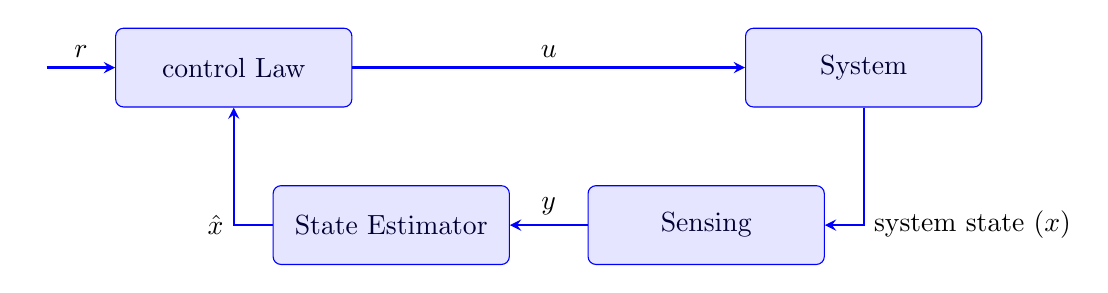
\begin{tikzpicture}[node distance=2cm]
        \node (in) [eNode] {};
        \node (control) [recNodeB, right of=in, xshift=0.5cm] {control Law};
        \node (sys) [recNodeB, right of=control, xshift=6cm] {System};
        \node (sensor) [recNodeB, below of=sys, xshift=-2cm] {Sensing};
        \node (estimator) [recNodeB, below of=control, xshift=2cm] {State Estimator};
        
        \draw [arrowB] (in) -- node[above] { $r$} (control);
        \draw [arrowB] (control) -- node[above] { $u$} (sys);
        \draw [arrowB] (sys) |- node[right] { system state ($x$)} (sensor);
        \draw [arrowB] (sensor) -- node[above] { $y$} (estimator);
        \draw [arrowB] (estimator) -| node[left] { $\hat{x}$} (control);
    \end{tikzpicture}
    
    \caption{A typical feedback control loop where the physical plant (\textit{System}) is monitored via an array of sensors (\textit{Sensing}) which produce noisy sample of the state variables $y$. 
    And after sensing, \textit{State Estimator} aggregates the measurements from all the sensors and produce estimation of the current state $\hat{x}$. Then the \textit{Control Law} produce output to the actuators ($u$) in order to close the gap between the current estimated state and the reference state ($r$).
    \label{fig:control loop}}
\end{figure}

\section{The proposed approach} % (from paper)
\label{sec:architecture}

%TODO - verify we are not lying here
As proposed in earlier work on automata based scheduling (\cite{weiss2007automata,RTComposer,AW08}) we aim at a development process where a system is built as a composition of a set of components where each component is a software module (a set of procedures) accompanied with an automaton. Our addition here is that we allow the automata to be guarded, i.e., each automaton acts as a specification of a reactive system that tells the scheduler which functions of a component it may run in each slot depending on the \textbf{dynamic state} of the controllers. A second addition is that we have implemented the approach as an enhancement of the internal scheduler of the ArduPilot Mega (APM)~\cite{APM} open source unmanned vehicle autopilot software suite. A third contribution of this thesis is a proposal of a specific way to use the automata based scheduling framework with a Kalman filter. We elaborate on each of these in the following subsections:

\todo{Explain that we are proposing to focus on sensors (and actuators). The separation principle. Alignment with the structure of the ArduPilot and other controller codes.} 


\subsection{Architecture}
% TODO: Use the terminology of the figure

In our methodology, we use rich component specification represented by automata.
As presented above, the first advantage of this technique is the ability of the scheduler to ``react'' the state of the system, therefore we need more intense interaction between the \textit{Scheduler} and the control loops in particularly with the estimator.
The architecture of control system as we believe, is illustrated in Figure~\ref{fig:general_hybrid_loop}.
The architecture, that is based on modern controller architecture where the system has multiple controlling tasks, comes to support an efficient scheduling protocols in modern control systems consisting of a processor that runs all the tasks of many independent control loops in the system. 
Each control loop (blue components in Figure~\ref{fig:general_hybrid_loop}) will tell the \textit{scheduler} of its level of certainty ($P = var(\hat{x} - x)$) and the scheduler will allocate resource (processor time) based on this data, meaning the \textit{scheduler} allocate resource dynamically based on the system current needs rather than the worst case needs, making the scheduler an active part of the control loop.

%TODO - probably need to be in the Tests section
Our methodology is general and may be applicable in a wide range of applications. However, in this initial phase of the research, we focus on a specific sub-domain and in handling all technical issues in order to prove the concept.
%In this thesis we develop and implement a vision based controller for drone (see Section~\ref{sec:tests}) and analyze the concept with it.

\begin{figure}[h]
    \centering
    
    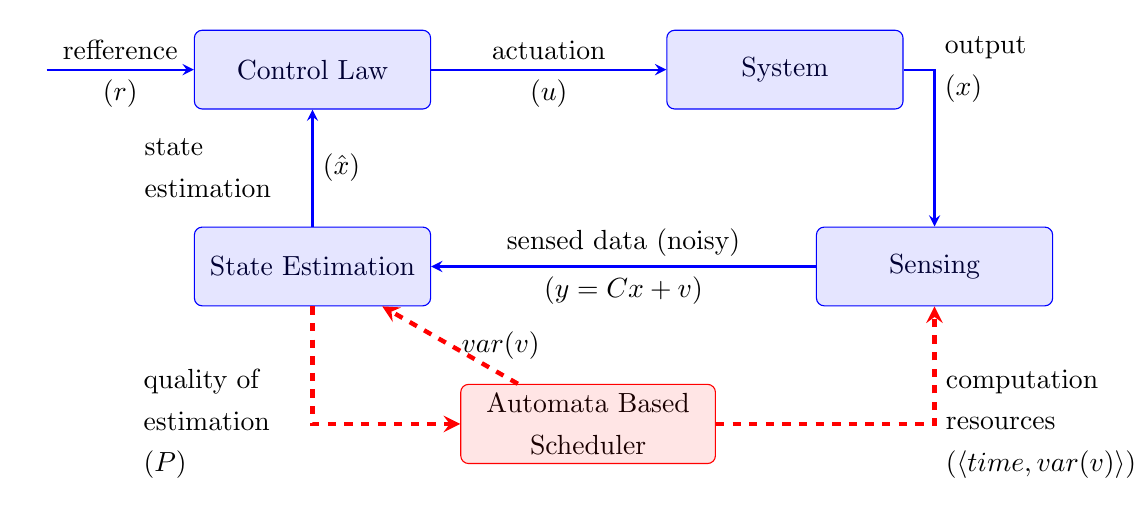
\begin{tikzpicture}[node distance=2cm]
    \node (in) [eNode] {};
    \node (control) [recNodeB, right of=in, xshift=1.5cm] {Control Law};
    \node (sys) [recNodeB, right of=control, xshift=4cm] {System};
    \node (sensor) [recNodeB, below of=sys, xshift=1.9cm, yshift=-0.5cm] {Sensing};
    \node (estimator) [recNodeB, below of=control, yshift=-0.5cm] {State Estimation};
    \node (sched) [recNodeG, below of=estimator, xshift=3.5cm, text width=3cm] {Automata Based Scheduler};
    
    \draw [arrowB] (in) -- node[above] {refference} node[below] {($r$)} (control);
    \draw [arrowB] (control) -- node[above] {actuation} node[below] {($u$)} (sys);
    \draw [arrowB] (sys) -| node[right,text width=1cm] {output ($x$)} (sensor);
    \draw [arrowB] (sensor) -- node[above] {sensed data (noisy)} node[below] {$(y = Cx +v$)} (estimator);
    \draw [arrowB] (estimator) -- node[left,text width=2cm] {state \newline estimation} node[right] {($\hat{x}$)} (control);
    
    \draw [arrowG] (estimator) |- node[left,text width=2cm] {quality of estimation ($P$)} (sched);
    
    \draw [arrowG] (sched) -| node[right,text width=2cm] {computation resources ($\langle time,var(v) \rangle$)} (sensor);
    %\draw [arrowG] (sched) -| node[right] {$\langle time,var(v) \rangle$} (sensor);
    
    \draw [arrowG] (sched) --  node[right] {$var(v)$} (estimator);
    
    \end{tikzpicture}
    
    \caption{The controller framework we implement, Each control loop (depicted in blue) informs the resource allocator (Scheduler) of its quality of estimation, the \textit{scheduler} will allocate CPU time accordingly in order to maintain valid estimation quality. 
        Specifically for the Sensing processes, for example in our case \textit{Computer Vision} task, the guard automaton specify the required sensing quality ($var(v)$) which determines the required execution time ($time$). The Sensing alocation is noted by $\langle time,var(v) \rangle$.
        %The underlying assumption here is that the noise in the sensed data is a function of the amount of computation resources. We assume that the more resources are invested in sensing the better (less noisy) sensed data is obtained.
        \label{fig:general_hybrid_loop}}
\end{figure}

\subsection{Guarded Automata as Interfaces for Control and Scheduling}
As our goal is to allow dynamic selection of the computation load in the feedback loops based on the states of the systems, we start with a general software architecture in which each component (implementation of a specific feedback loop) is represented by a code module (in our case, a class in C++) and an automaton that specifies when to invoke its methods. The transition relation of the automaton depends, in addition to the current state, also on data produced by the estimator of the feedback loop (we experimented with different options for this data, as discussed below).

The motivations of using automata as described above are: (1) Automata allow for a rich specification language; (2) It is easy to construct schedules that obey the specification with negligible computational burden; (3) Automata theory gives a solid framework for composing the specifications of competing requirements for analysis and for schedule synthesis. 

%TODO - mybe reference to future work section
In this thesis we focus on the first two motivations in the above list. The third is discussed in details in earlier works on automata based scheduling and is the focus of future paper that we are preparing where we describe some analysis techniques we have developed for guarded automata.   

\subsection{Implementation in an Auto Pilot Software}
As our main case study is in flight control (see Section~\ref{sec:caseStudy}), we chose the ArduPilot Mega (APM) platform for experiments~\cite{APM}. To this end, we implemented a basic automata based scheduler for this platform. The built-in task scheduling specification in APM consist of a table as shown in Figure~\ref{fig:apm-scheduler}. This table is easy to maintain and to adjust, but it is used under an assumption that there is enough CPU power to run all the tasks in the specified frequencies. APM does contain a mechanism to handle overruns, by moving tasks to the next window when there is not enough time to run them now, but the system is designed under the assumption that this only happen in rare situations.
%TODO - maybe add APM section in apendex describing this scheduler with image

To allow a reactive scheduler that runs different modes of the software-based controllers depending on their state, we replaced the scheduling table in our version of the APM with automata that specify when to run the tasks. Note that automata allow for specifying the requirements that the table represents, using simple circular automata without guards (see, e.g., \cite{weiss2007automata}). Automata, however, can model more advanced scheduling instructions with very little addition to the complexity of the scheduler, as we will demonstrate in Section~\ref{sec:simulation} and in Section~\ref{sec:caseStudy} below.
%TODO - were gose the detail of the automaton operations

\begin{figure}[]
    \scriptsize
    \begin{lstlisting}
    /*
    scheduler table - all regular tasks apart from
    the fast_loop() should be listed here, along 
    with how often they should be called (in 10ms 
    units) and the maximum time they are expected 
    to take (in microseconds)
    */
    static const AP_Scheduler::Task 
    scheduler_tasks[] PROGMEM = {
    { update_GPS,            2,     900 },
    { update_nav_mode,       1,     400 },
    { medium_loop,           2,     700 },
    { update_altitude,      10,    1000 },
    { fifty_hz_loop,         2,     950 },
    { run_nav_updates,      10,     800 },
    { slow_loop,            10,     500 },
    { gcs_check_input,       2,     700 },
    { gcs_send_heartbeat,  100,     700 },
    { gcs_data_stream_send,  2,    1500 },
    { gcs_send_deferred,     2,    1200 },
    { compass_accumulate,    2,     700 },
    { barometer_accumulate,  2,     900 },
    { super_slow_loop,     100,    1100 },
    { perf_update,        1000,     500 }
    };
    \end{lstlisting}
    \caption{APM scheduling specification}
    \label{fig:apm-scheduler} 
\end{figure}

\subsection{Integration With a Kalman Filter}
The third layer of the approach we propose is based on the observation that a standard Kalman filter produces information that can be used to guide the automata of the components. 

As we will elaborate in the description of the simulations and of the case study below, we propose to schedule the functions that implement algorithms for sensing and for actuation based on the error variance of the estimation that a Kalman filter provides, the idea is to operate different sensing modes in order to regulate the estimation error variance, see Section~\ref{sec:kalman} for Kalman-filter characteristics. 
\todo[inline]{ maybe add paragraph with details and examples in the real word: changing in dayligth surface texture...}
\todo[inline]{we can show diferent prespectives: 1. offline scheduling using only $P$ (eror covariance matrix), 2. online scheduling using $\tilde{y_k|k}$ with the explenation that in the real world the errors are not always normal.}


%In this framework the scheduler is part of the control logic and therefore it can make scheduling decisions based on the current control state, the scheduling of \textit{Computer~Vision} task depends on the accuracy of state estimation.
%For example, if the vision is clear, the \textit{Computer~Vision} will produce good measurement of the \textit{System} and therefore good accuracy will be achieved so the \textit{Scheduler} can allocate less computation time to the heavy \textit{Computer~Vision} task and still remain stable while allocating more CPU to others control loops or to background tasks (like navigation).

\section{A demonstration of the approach in simulation}
\label{sec:simulation}
%TODO - explain that we developing an idea that culd in the future become a tool

Our approach for using automata for scheduling resources in software based controllers is based on the observation that in most systems the computational load is in the implementation of the sensors and actuators, not in the implementation of the controllers that usually consist of quick arithmetic manipulation of a small amount of variables. We therefore focus our attention on allowing a trade-off between CPU usage of sensors and actuators and their accuracy. %In this work, as a main motivating example, we focus on the case of visual sensors that employ image processing algorithms.

As said in Section~\ref{sec:architecture}, we propose to implement the resource scheduling decisions using automata that control which procedures are invoked in the control loops. More specifically, for sensors or actuators that require heavy computations, such as vision based sensors, we propose that the software engineers develop several modes of sensing, each consumes a different amount of CPU and provides a different level of accuracy. 

\todo{not realy like the actuators here, they are not really modeled. we consider they error as ``process error'' }
Formally, we assume that each of the physical processes we control is a Linear Time Invariant (LTI) system with a known model, as depicted in Figure~\ref{fig:simulink}. The inaccuracies of the sensors and of the actuators are modeled as additive Gaussian noise with a known variance. As a basis for scheduling, we assume that each sensor (and, possibly, also the actuators) can be scheduled to operate in one of a range of modes at each computation slot, each mode consuming a certain percentage of the CPU and giving a certain variance of the measurement (or actuation) noise.

\begin{figure}%[htbp]
    \centerline{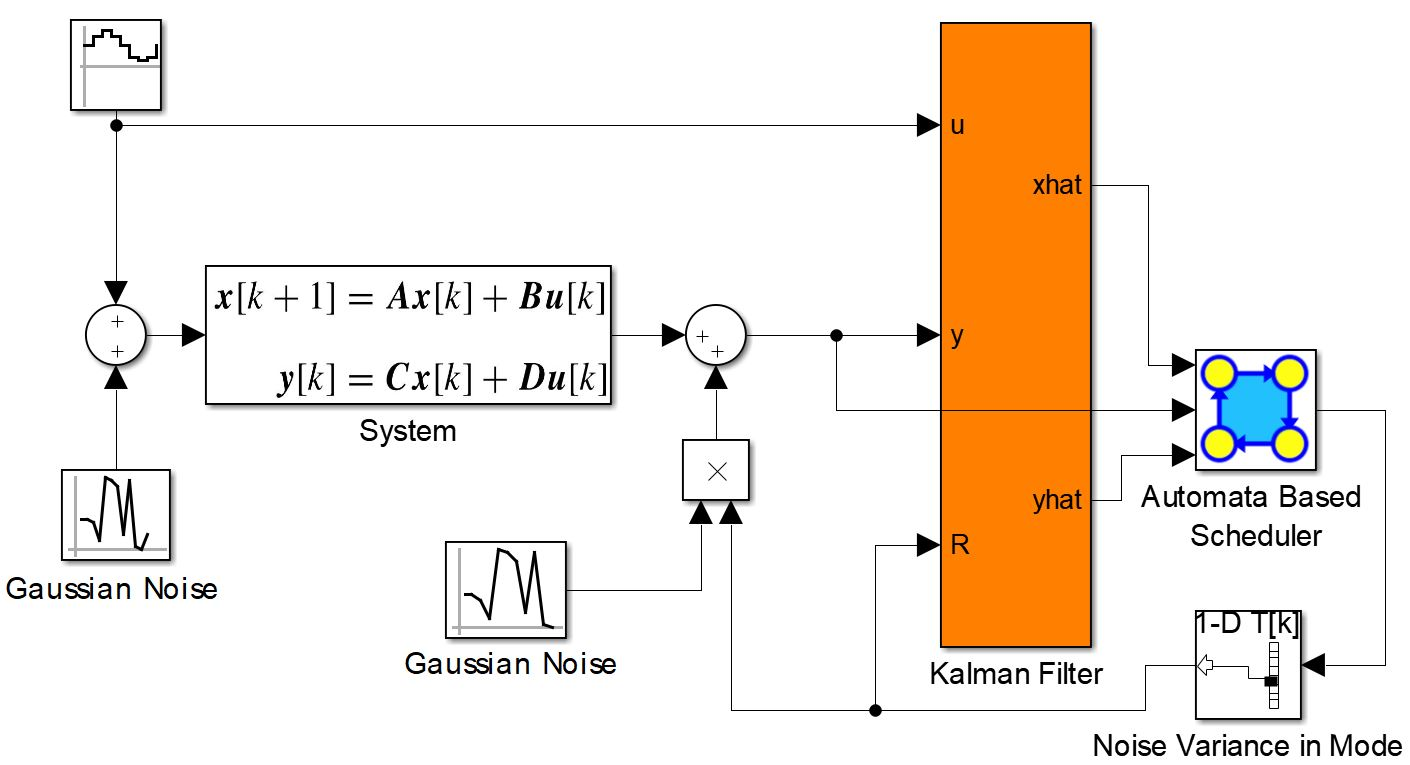
\includegraphics[width=100mm]{SimulinkModel.jpg}}
    \caption{A Simulink model used to demonstrating and  examine the proposed approach.}
    \label{fig:simulink}
\end{figure}

The scheduling of the modes, for each of the components, is governed by the automata based scheduler as depicted in Figure~\ref{fig:simulink}. We propose to use a standard Kalman filter as a tool to gather the information that guides the state evolution of the automata, as follows. The filter gets as input the actuations ($u$),  measurements ($y$), and the covariance matrix of the measurement noise ($R$). We assume that the measurement noise is a static function (represented here as a translation table) of the mode chosen by the scheduler. The output of the Kalman filter is fed to the scheduler that uses it for advancing the states of the automata. 
In the Simulink model depicted in Figure~\ref{fig:simulink}, the covariance matrix of the disturbance, which in this case is $1 \times 1$ matrix consisting of the noise variance, is fed to the Kalman filter (as its $R$ input) and to the block that multiplies the Gaussian noise by the variance (the product of a white noise with unit variance and a constant $v$ yields a Gaussian noise with variance $v$).

We ran the model depicted in Figure~\ref{fig:simulink} with the linear time invariant system
\begin{eqnarray*}
    x(k+1) &=& \begin{pmatrix}        1.3  & -0.5  & 0.1 \\
        1    & 0     & 0 \\
        0    & 1     & 0
    \end{pmatrix}x(k)+ 
    \begin{pmatrix}
        -0.4 \\
        0.6\\
        0.5\end{pmatrix} u(k) \\
    y(k)&=& \begin{pmatrix}1 & 0 &0\end{pmatrix}x(k)
\end{eqnarray*}
taken from \url{mathworks.com/help/control/examples/kalman-filter-design.html}. As seen in Figure~\ref{fig:simulink}, we injected a sinusoidal input (with $amplitude=bias=frequency=1$) to this system. 
The actuation noise, depicted on the left, is with a unit variance. 

The `Automata Based Scheduler' block is designed to set the variance of the sensing noise dynamically to be either $0.25$ or $1$ at each step of the simulation. This models a sensor that has two modes of operation: a mode with high accuracy, that produces normally distributed measurement errors with low variance, and a mode with low accuracy that produces normally distributed measurement errors with higher variance. We assume, for the performance measurements presented below, that the CPU consumption of each mode is $\%CPU=1.1-errVar$, where $errVar$ is the variance of measurement errors in the mode.

We ran this model with three versions of the `Automata Based Scheduler' block. The first version, called `High' in Table~\ref{tbl:sim-results}, is where the block acts simply as the constant $1$, ignoring its inputs altogether. Similarly, the term `Low' in the table refers to an implementation where the block is the constant $0$. These two implementations model the constant schedules, where the sensor is operated in one mode along the whole execution. These two schedules are compared to a third implementation, called 'Aut. Based' in the table, where the block implements the schedule given by the automaton:
\begin{center}
    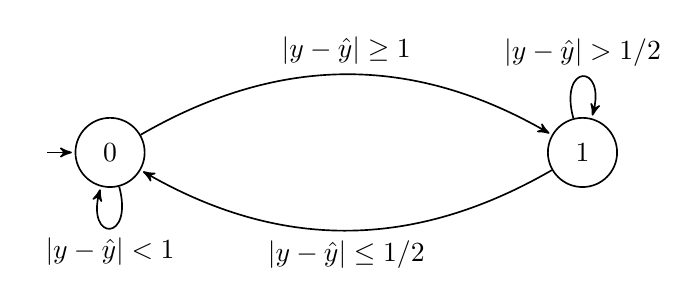
\begin{tikzpicture}[->,>=stealth',shorten >=1pt,auto,node distance=6cm,
    semithick]
    
    \node[initial,state] (A)                 {$0$};
    \node[state]         (B) [right of=A]    {$1$};
    
    \path (A) edge [bend left]             node {$|y-\hat{y}|\geq1$} (B)
    (A) edge [loop below] node {$|y-\hat{y}|<1$} (A);
    
    \path (B) edge [bend left]             node {$|y-\hat{y}|\leq 1/2$} (A)
    (B) edge [loop above] node {$|y-\hat{y}|>1/2$} (B);
    
    \end{tikzpicture}
\end{center}
The states of the automaton represent operation mode of the sensor, 0 for `Low' mode and 1 for `High' mode.
$|y-\hat{y}|$ means how far is the last measurement from the expected measurement this value act as indication (and consider approximation) of the overall real noises, process, measurement and actuation noises together.
The automaton try to formalize the expression: ``use `High' mode only after observing high distributed''.

%A = [1.1269   -0.4940    0.1129,
%1.0000         0         0,
%0    1.0000         0];
%
%B = [-0.3832
%0.5919
%0.5191];
%
%C = [1 0 0];

\begin{table}
    \centering
    \begin{tabular}{ |  l  | c | c | c | }
        \hline
        &  High & Low & Aut. Based \\ \hline \hline
        \%CPU                    & 85 & 10  & 46 \\ \hline
        mean of $|x -\hat{x}|$ & 0.97 & 1.24 & 1.08 \\ \hline
    \end{tabular}
    \caption{Simulation results.}
    \label{tbl:sim-results}
\end{table}

The results of the simulation, summarized in Table~\ref{tbl:sim-results}, show, as expected, that the CPU consumption is much lower (0.1) when using the low-quality version of the sensing algorithm and is higher (0.85) when the high-quality version of the sensing algorithm is used. The performance of the estimation, in terms of the mean distance between $x$ (the real state) and $\hat x$ (the Kalman filter estimated state), is better with the high-quality version (0.97) than it is with the low-quality version (1.24). More interestingly, we can see that the experiment with the automaton that switches between the two sensor modes yields performance that is close to the performance of the high-quality sensing algorithm, using much less CPU. This demonstrates how automata based reactive scheduling can allow for new ways to balance performance and computational resources in software based controllers. 

\section{Case Study: Stabilizing a Quad-rotor in Front of a Window}
\label{sec:caseStudy}
% overview of why we use vision example

The case study we used to test our concept is the development of a controller that stabilizes a quadrotor in front of a window (see, e.g.,~\url{rpg.ifi.uzh.ch/aggressive_flight.html}).
We implemented an autonomous controller for that task and evaluated its performance.

The part of the controller that we focused on is the vision based position controller. Specifically, the main controller, that we will describe below, uses a standard low-level angular controller and a simple image processing algorithm that identifies the position of the corners of the window in the image plane\footnote{In the experiment, to simplify the image processing algorithm, we marked the corners of the window with led lights.}. Its goal is to regulate the position of the quadrotor by tilting it. Note that rotations of the quadrotor by a small angle generate a more-or-less proportional accelerations in a corresponding direction, hence we can approximate the system with a linear model. A main challenge for this controller is that the computer vision algorithm takes significant time to compute relative to the fast control loop. We can decrease computation time by lowering the resolution, but this also increases the measurement noise. We will demonstrate how reactive scheduling of the resolution can serve for balancing resource consumption vs. control performance in this system.

\subsection{Observer Design}
\label{sec:Observer Design}
We first implemented an observer based on the work of Efraim~\cite{Efraim17}. The observer gets the positions of the widow corners from the image (see Section~\ref{sec:Experiment setup} for more details), %enumerated clockwise starting from the top left corner noted by $p_1,p_2,p_3,p_4$, 
and extracts the following four quantities based on the shape and location of the window corners in the image plane: %$S_x$, $S_y$, $V_d$ and $sz$, as follows.
\textbf{Center of mass:} $S_x$ and $S_y$ represent the window ``center of mass'' along the $x$ and $y$ axes of the image, respectively, normalized to the range of $[-1,1]$.
These values are used for controlling the yaw angle and the altitude of the drone, respectively. Means the drone is always facing the center of the window and at the altitude of the center of the window. 
\textbf{Window size:} $sz$ is the sum of the vertical edges of the window. It is used to measure the distance of the drone from the window~\footnote{We used a fixed size window and converted $sz$ to distance (in meters in our case) based on the size of the window. In the general case the units of distance are relative to the window size.}.
\textbf{Vertical difference:} $V_d = {((y_1-y_4)-(y_2-y_3))}/{((y_1-y_4)+(y_2-y_3))}$, were $y_i$ is the vertical position of the widow corners in the image in the range of $[-1,1]$, enumerated clockwise starting from the top left corner. It is measure the angular position of the drone in relation to the window (parallel to the ground) and used to control the position of the drone among the $x$ axis.
Note that although $V_d$ is not directly measure the linear $x$ position of the drone, we can estimate the linear $x$ position by simple geometry:
as show in Figure~\ref{fig:V_d-geomerty} $x = l * \sin (V_d)$ were $l$ (distance from window) can be calculated from $sz$. I our case because $V_d$ is usually relatively small we approximate it by $x = l * V_d$.

% TODO add fig:V_d-geomerty
\begin{figure} %[htbp]
    \centerline{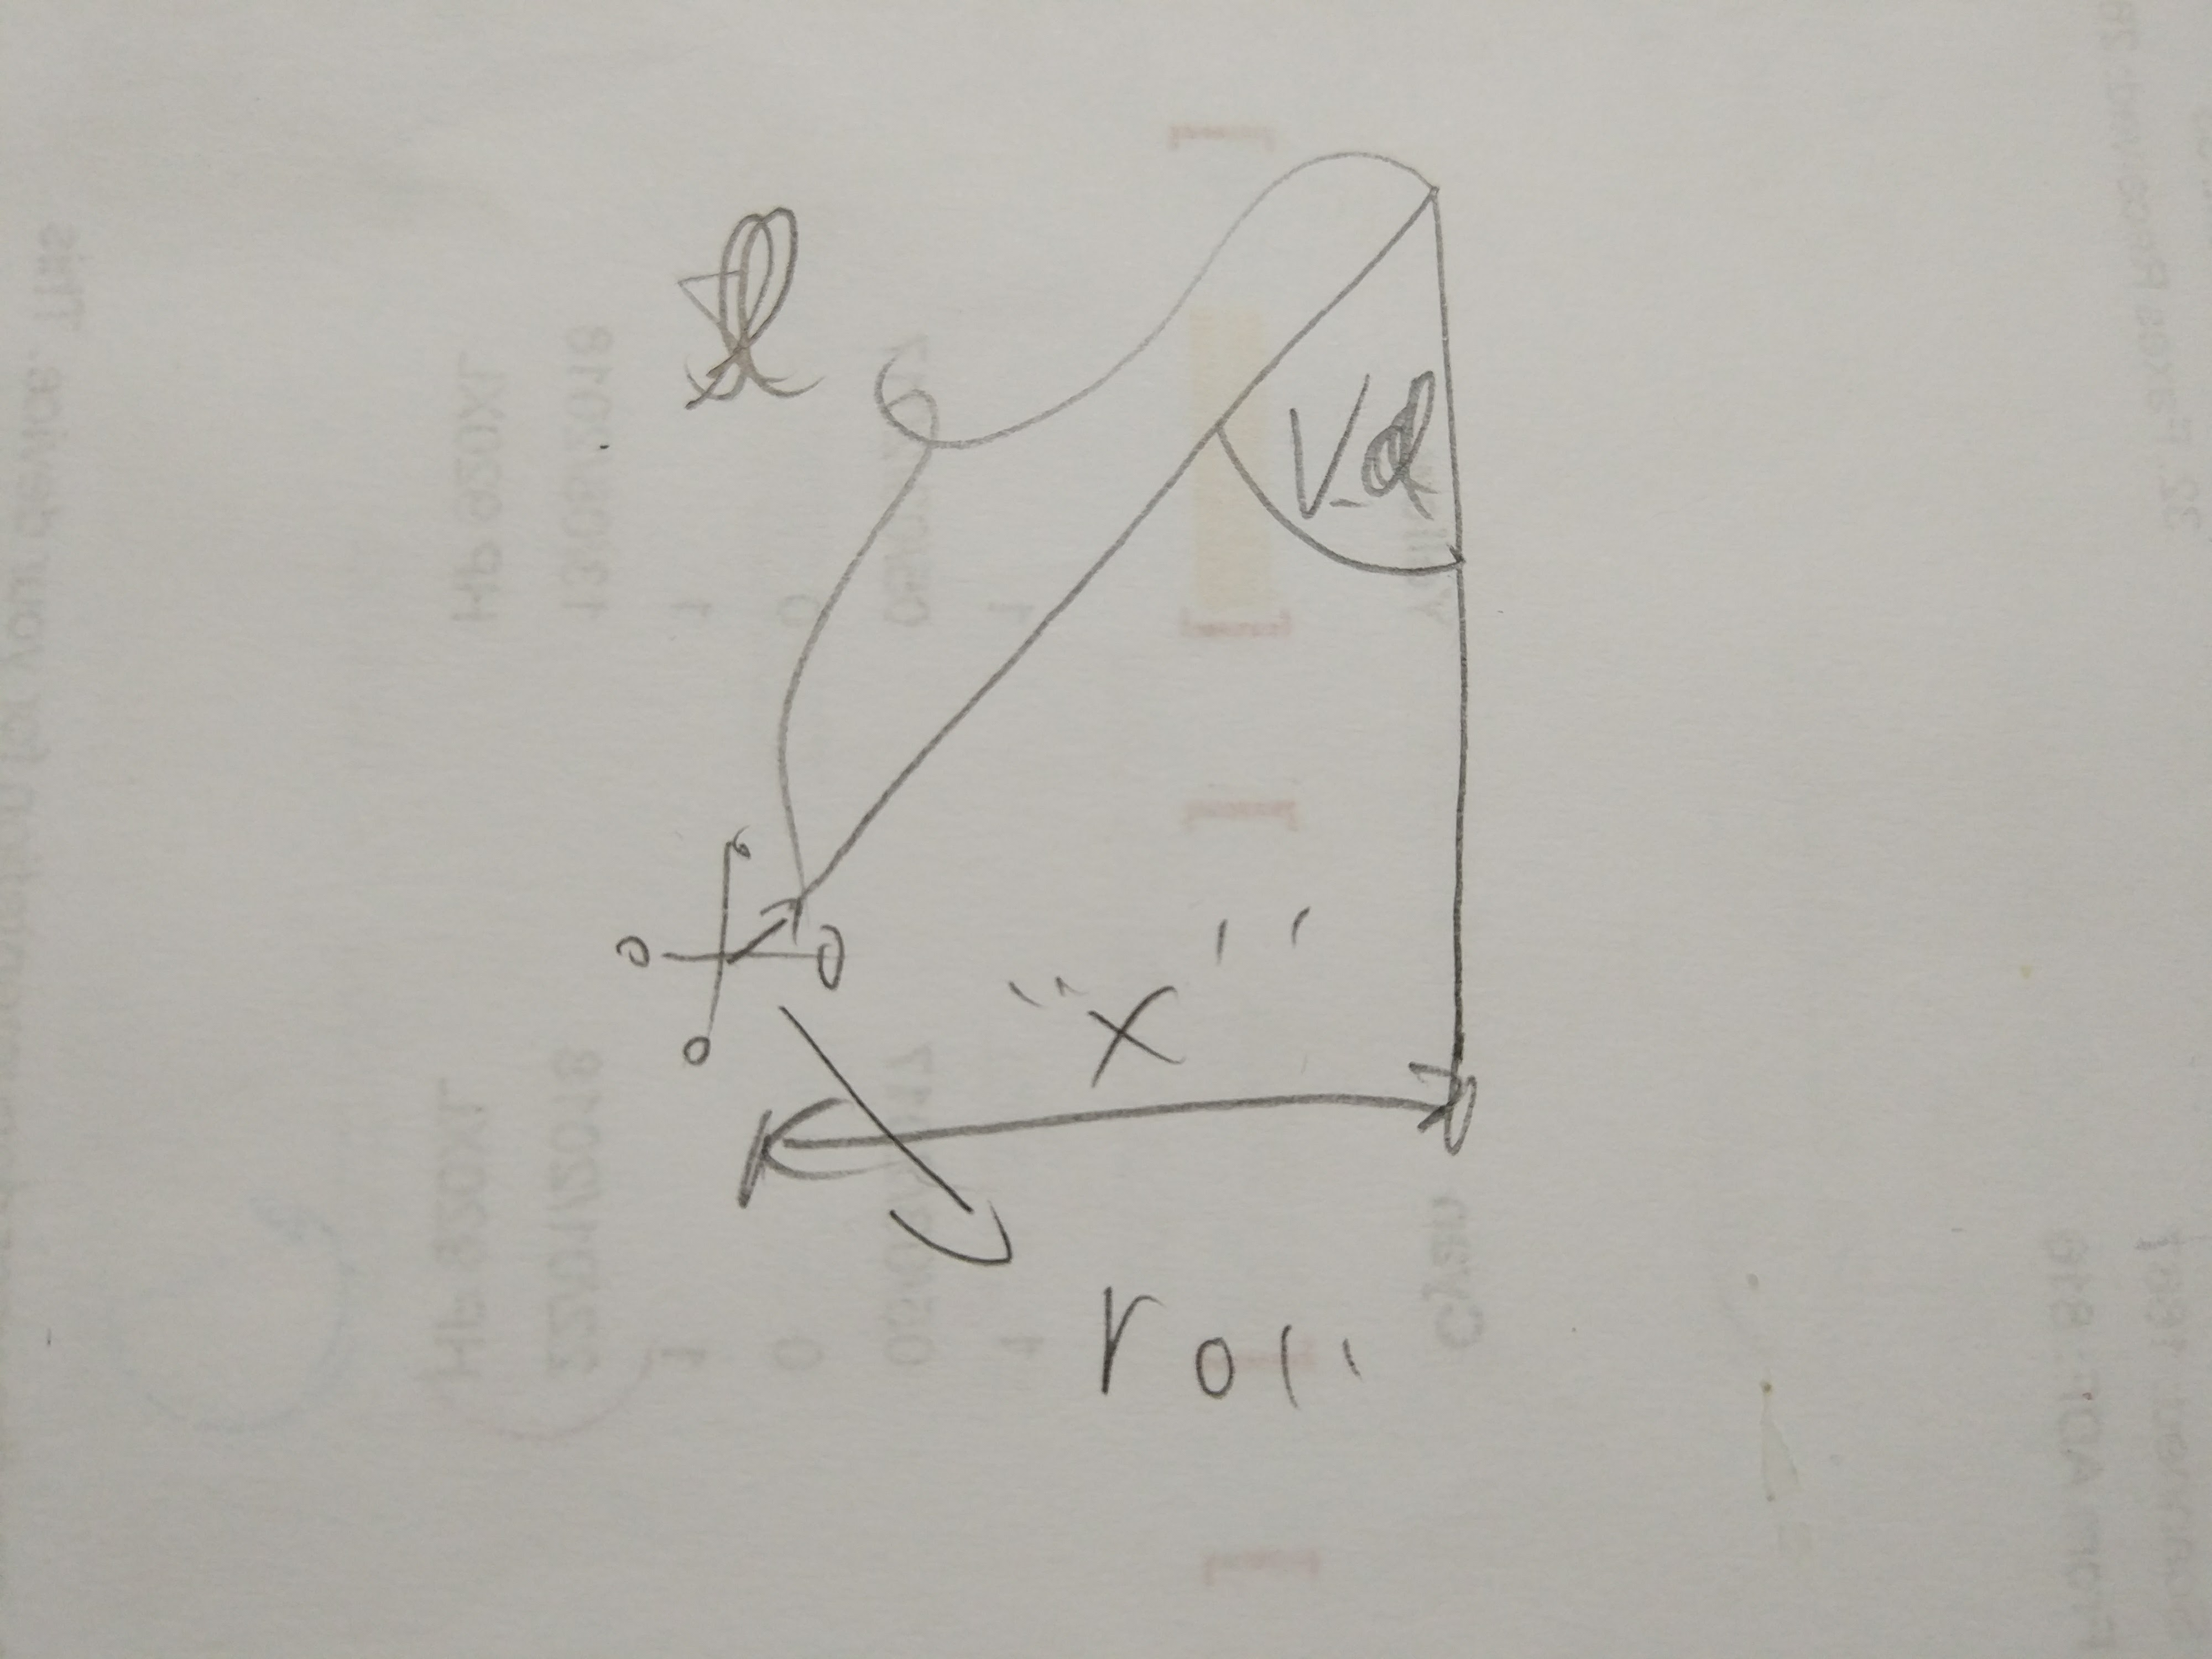
\includegraphics[width=80mm]{vd-geometry.jpg}}
    \caption{Geometric relation between $\alpha$ (the angle derived from $V_d$) $l$ (distance from window extracted from $sz$) and the position of the drone among the $x$ axis. (TODO - need to replace image)}
    \label{fig:V_d-geomerty}
\end{figure}

\todo{don't know if some of this need to be moved to Section~\ref{sec:kalman}}
As common in engineering practices, we pass these numbers to a filter that gives us a more informed state estimation. 
In theory, as demonstrated in the simulation in Section~\ref{sec:simulation}, we should use Kalman filter estimator for best state estimation. As we deal with a non-linear system here, and because the process noise distribution is not known (it is significantly affected by the varying state of the battery), and because Kalman filter adds complexity in the code, we use a complementary filter.
A complementary filter is actually a steady-state Kalman filter for a certain class of filtering problems~\cite{complementaryVSKalman}.
Specifically, in our case study, we implemented a two steps estimator that: (1) \textit{predicts} the current state evolved from the previous state (denoted by $\hat{x}_{k|k-1}$) using a linearized model of the system, and then \textit{updates} the prediction with current state measurement from the image, denoted by $y_k$.
The result of the estimation, denoted by $\hat{x}_{k|k}$, is a complementary filter of the prediction ($\hat{x}_{k|k-1}$) and the measured state ($C^{-1}y_k$)~\footnote{The matrix $C$ is the measurement matrix as shown in the model at Figure~\ref{fig:simulink}}:
$ \hat{x}_{k|k} = K \hat{x}_{k|k-1} + (1-K) C^{-1}y_k $ were $K$ is constant that equals the Kalman filter gain ($K_k$) at a steady-state, see Section~\ref{sec:kalman} for detail information.
\todo[inline]{need to add section on the system linearized model?}

The image processing algorithms can run in different operation modes, each mode with different accuracy (see Section~\ref{sec:Analysis}).
The constant $K$ represents the ratio between the variance of the process noise and the variance of the measurement noise. To achieve best performance, we define a separate value of $K$ for each mode.

\begin{figure} %[htbp]
    \centerline{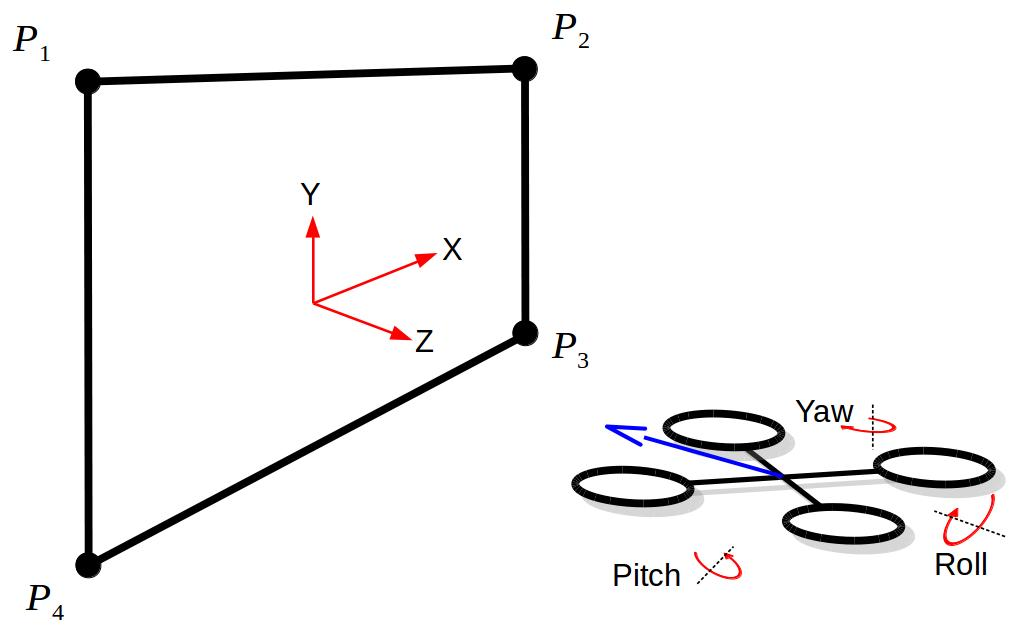
\includegraphics[width=100mm]{axis.jpg}}
    \caption{The coordinate system and the rotation axes of the drone, the position axis ($x$, $y$ and $z$) are in relation to the window, ``Yaw'' angle is the horizontal angle of the center of the window related to the front of the drone, ``pitch'' and ``roll'' are angles of the drone itself (calculated from the inertial sensors only).}
    \label{fig:axis}
\end{figure}

\subsection{Controller Design}
\label{sec:Controller Design}

In this experiment, we consider the task of hovering in front of the window. The controller objective is to hover parallel to the window (center of $z$ axis in Figure~\ref{fig:axis}) at the altitude of the window within distance of two meters in front of the window ($y=x=0 , z=2$) and face pointed to the center of the window (yaw angle).
We consider this point as the desire reference position and the coordinates are according to Figure~\ref{fig:axis}.

The controller consists of four independent feedback loops: altitude, yaw, pitch, and roll.
The pitch and the roll controllers are copies of the same attitude controller which gets as input the required pitch or roll angel, respectively. These controllers runs in parallel to a position controller that maintains the required distance ($z$ position) and displacement ($x$ position) relative to the window, the position level controller outputs the required angle (acceleration) to the attitude controller as show in Figure~\ref{fig:controllerStracture}.
Altitude, yaw and $x$ and $z$ position is regulated relative to the window.
The inertial pitch and roll feedback for the low level controllers is related to the drone body and is generated by the existing \textit{Attitude and Heading Reference system} (AHRS) library of ArduPilot (see Section~\ref{sec:Experiment setup}) and the position feedback ($x$, $y$, and $z$ position) came directly from the observer described in Section~\ref{sec:Observer Design}.

\begin{figure} %[htbp]
    \centerline{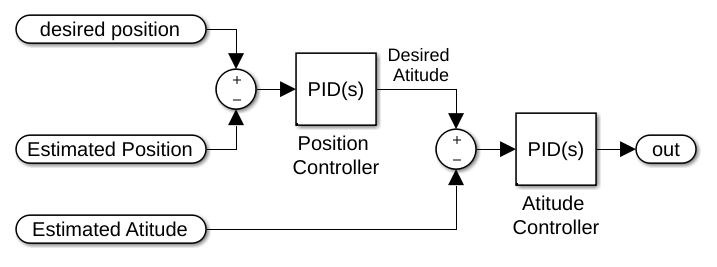
\includegraphics[width=100mm]{two_level_controller.jpg}}
    \caption{Attitude and position controller consisting of a two level, cascaded, structure.}
    \label{fig:controllerStracture}
\end{figure}

%TODO - some conversion proof
The position controller is as follows:
The altitude ($y$ position) is obtained directly from the $S_y$ value explained in Section~\ref{sec:Observer Design} and it is regulated by changing the overall ``throttle'' of the rotors, this is good approach assuming the drone pitch and roll angles are close to zero then $S_y$ is almost proportional to the real altitude of the drone and the trust vector is pointed up.
The $z$ position is assumed to be the distance from the center of the window and is calculated as proportional to the window size $sz$ value, it is regulated by changing the pitch angle. Assuming the drone is always facing the center of the window (yaw angle is zero) the pitch angle produce acceleration to the pitch direction that is to the window direction or from the window meaning its will decrise or increase the $z$ position.
The $x$ position (displacement) is regulated by changing the roll angle. Similar to $z$ position, assuming the drone is always facing the center of the window the roll angle produce acceleration that increase or decrease the $x$ position depending on the roll angle direction.

As demonstrated in Figure~\ref{fig:acceleration_static_diagram}, the $x$ acceleration is equal to $a_x=g \arctan(\alpha_{roll})$ and $x$ acceleration is equal to $a_z=g \arctan(\alpha_{pitch})$. 
In practice, during this work we usually assume linear proportional acceleration meaning $a_x=g \cdot \alpha_{roll}$ and $a_z=g \cdot \alpha_{pitch})$.

Note that if $x$ is not zero then the drone is not parallel to the window and the roll direction (that used to regulate $x$ position) is also affects the $z$ position.
Similarly, if the drone is not parallel to the window and the pitch direction (that used to regulate $z$ position) is also affects the $x$ position.
Although in theory $x$ controller interrupt the $z$ controller and vice versa, in practice even if the drone displacement is relatively large, when all the controllers executed together thy constantly fix those side-afects and because the $x$ position is generally decreased during this process we eventually converge to a stable state were the drone is near-parallel to the window.

%TODO add fig:acceleration_static_diagram
\begin{figure} %[htbp]
    \centerline{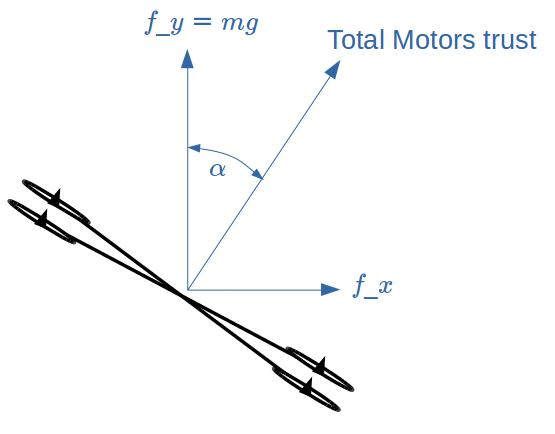
\includegraphics[width=50mm]{acceleration_static_diagram.jpg}}
    \caption{Free body diagram (force diagram) of the drone $x-y$ or $z-y$ plane forces, this diagram demonstrate the relation between $x$ or $z$ aceleration ($a_x$ or $a_z$) and the corresponding tilt angle. $\alpha$ represent the tilt angle (roll or pitch) and $a$ represent the acceleration in the corresponding direction. We assume that the altitude controller work as expected and the vertical speed is close to zero ($a_y = 0$), and we get $m a = \arctan(\alpha) mg$, that is, the acceleration is $a = \arctan(\alpha) g$ we use tis relation for the controller design (Section~\ref{sec:Controller Design}) and we also use this calculation as part of the system model in the Observer (Section~\ref{sec:Observer Design}) }
    \label{fig:acceleration_static_diagram}
\end{figure}

Based on the \textit{principle of separation of estimation and control}, we can use that controller regardless of the measurement quality. We implemented a basic Proportional Integral Derivative (PID~\cite{aastrom2006advanced}) controller and tuned the parameters by trial and error using the highest resolution observer.

%%%%%%%%%%% Specification Automata %%%%%%%%%%%%%
\subsection{Analysis and Specification Automata}
\label{sec:Analysis}

The objective of the system is to maintain stable hovering in front of the window, performances is measured by the amount of deviation from the center line of the window in the critical axis $x$, i.e., we want to minimize $\left| x \right|$ (see Figure~\ref{fig:axis}).
Our goal is to achieve maximum performance with minimal amount of processing time.
Obviously, both goals cannot be achieved together. We therefor aim at achieving a good trade-off between processing resources and quality of measurement. The focus is on the main consumer of computation resources: the image processing algorithm.
We aim at taking resources (high CPU time) only when needed. By this, we will reduce the average CPU usage without significantly affecting the performance.
Specifically in our case study, we switch between camera resolutions dynamically during the flight. The observer modes, discussed above, correspond to image resolutions (see Section~\ref{sec:Observer Design}).
For simplicity, we consider in this thesis only two modes: \textit{High quality} with resolution of 960p and \textit{Low quality} with resolution of 240p.

Looking at the test results shown in Table~\ref{tab:results}, we see that the high quality observation mode provides mean error tolerance of 9.5\textit{cm} (in the $x$ axis) with the cost of 30\% CPU usage.
On the other hand, the low quality mode provides mean error of 30\textit{cm} (three times the error obtained in the high quality mode) using only 2.1\% CPU usage~\footnote{The CPU usage percentage is the average: (total time spend in image processing)/(total flight time). }.

We explain next several approaches we applied in the design of a \textit{reactive scheduling specification} that combines the both high and the low resolution sensing modes in an sufficient way.

%displacement ($x_{k|k}$) schedulers
We first examined a straight-forward scheduler based directly on the current position (the $x$ axis of $\hat{x}_{k|k}$). Using the simple guarded automaton $A_{x}$ presented in Figure~\ref{fig:test_automata}, we defined a dynamic observer that chooses the mode (high or low sensing quality) based on the absolute value of the $x$ axis of $\hat{x}_{k|k}$. If the drone is closer to the center line of the window, denoted by $|x| < T_x$, we consider it as a ``safe'' state and go to the mode called $L$ that schedules the low quality image.
Similarly, a state is considered ``BAD'' when the drone is far, denoted by $|x| > T_x$. In this case, we take high quality images in order to ``fix'' the state.
The threshold $T_x$ can be changed to tune the desired performances and processing time trade-off.
See Section~\ref{sec:results} for the data we collected by experiments to validate that this indeed achieves the required goals. 
% Results shows good improvement in term of resource utilization (see Section~\ref{sec:results}). 

%error ($y_{k|k}$) schedulers
In a second experiments set, we used the $A_{err}$ automaton presented in Figure~\ref{fig:test_automata}. This automaton is similar to $A_x$ with the difference that it switches states based on $\tilde{y}_{k|k}$ value  defined as:

\begin{dfn}{Measurement post-fit residual} 
    $\tilde{y}_{k|k}$, is the difference between the expected measurement, $C\hat{x}_{k|k}$, and the measured state, $y_k$: $\tilde{y}_{k|k} =  C\hat{x}_{k|k} - y_k $.%~\footnote{ Measurement post-fit residual $\tilde{y}_{k|k}$ is also defined by the Kalman filter.}.
\end{dfn}

The motivation to use this indicator comes form looking at the low quality experiment graph, shown in Figure~\ref{fig:testPlot}. We can see that $\left| \tilde{y}_{k|k} \right|$ growth is proportional to the deviation from the center of the window (in the $x$ axis). We can also see that the growth in $\left| \tilde{y}_{k|k} \right|$ precedes the growth in $x$. This means that we can use $\left| \tilde{y}_{k|k} \right|$ values to predict deviations in $x$.


In $A_{err}$ the observer operates in low quality when $\left| \tilde{y}_{k|k} \right| < T_{l}$ (``GOOD'' state) and switches to high quality when $\left| \tilde{y}_{k|k} \right| > T_{h}$ (``BAD'' state).
The thresholds $T_{l}$ and $T_{h}$ were initially taken from the low and the high quality graphs and fine tuned by experiments. 
Different $T_{l}$ and $T_{h}$ give different trade-offs of performances and processing time.
In Section~\ref{sec:results} we show that this dynamic observer gives almost the same performance as the high quality observer with a reduction of a factor of two in the processing load.

%complex / agregated schedulers (3-4 states)
The expressiveness of automata allows for creating even more complex scheduling specification. We can, for example, combine the approaches of both $A_{err}$ and $A_{x}$.
In Figure~\ref{fig:test_automata} there is two examples of such combinations. $A_{comp1}$ tries to save unnecessary CPU usage while the drone is in ``safe'' state, close to the center. It activates $A_{err}$ only if the drone goes far from the center ($T_{x}$cm from the origin).
$A_{comp2}$ adds another constraint: if the drone goes even farther away ($T_{x2}$cm from the origin) it schedules only high resolution to bring it back to safety.
The results show even better resource utilization.

\begin{figure}[htbp]
    \centerline{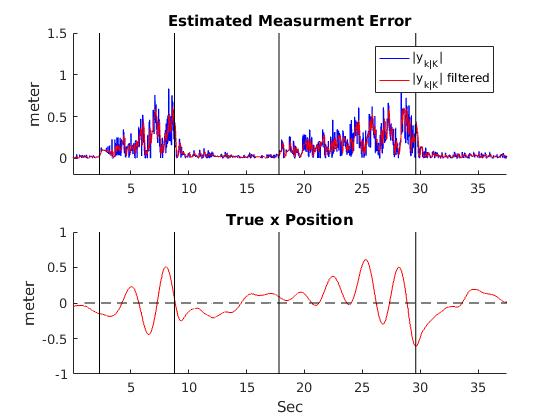
\includegraphics[width=100mm]{errorVsPosition.jpg}}
    \caption{This figure shows in the bottom plot the position of the quadrotor during the flight time and in the top plot the $\left| \tilde{y}_{k|k} \right|$ value during the flight. During the flight we manually switched between low and high resolution for further analysis. The modes (high or low) are separated by vertical lines, were the leftmost is high resolution then low and so on.}
    \label{fig:testPlot}
\end{figure}


%%%%%%%%%%%%%%%%%%%%%%%%%%%%%%%%%%%%%%%%%%%%%%%%%%
%%%%%%%%%%%%%%% automata %%%%%%%%%%%%%%%%%%%%%%%%%
%%%%%%%%%%%%%%%%%%%%%%%%%%%%%%%%%%%%%%%%%%%%%%%%%%
\tikzset{every edge/.append style={font=\small}}
\tikzset{every node/.append style={font=\small}}
\begin{figure} %[htbp]
    %\captionsetup{width=0.4\textwidth}
    \centering
    \begin{tabular}{c c}
        % by error
        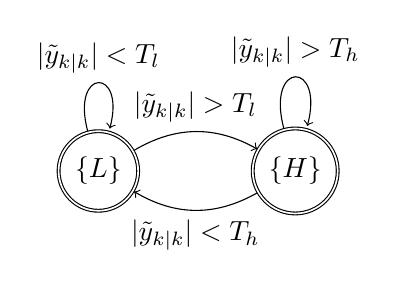
\begin{tikzpicture}[node distance=2.5cm,auto]
        \node (A) [state, accepting] {$\{L\}$};
        \node (B) [state, accepting] [right of=A] {$\{H\}$};
        
        \path[->] (A) edge [loop above] node {$|\tilde{y}_{k|k}| < T_l$} (A);
        \path[->] (A) edge [bend left] node {$|\tilde{y}_{k|k}| > T_l$} (B);
        \path[->] (B) edge [bend left] node {$|\tilde{y}_{k|k}| < T_h$} (A);
        \path[->] (B) edge [loop above] node {$|\tilde{y}_{k|k}| > T_h$} (B);
        %\path[->] (B) edge [bend left] node {$s_{0.7} \wedge est_1$} (A);
        \end{tikzpicture}
        
        &
        
        % by displacement (|x|)
        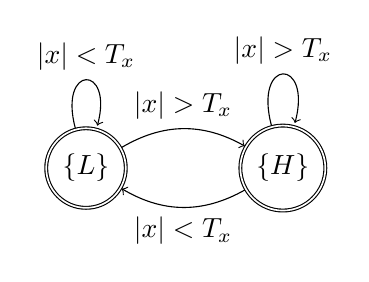
\begin{tikzpicture}[node distance=2.5cm,auto]
        \node (A) [state, accepting] {$\{L\}$};
        \node (B) [state, accepting] [right of=A] {$\{H\}$};
        
        \path[->] (A) edge [loop above] node {$|x| < T_x$} (A);
        \path[->] (A) edge [bend left] node {$|x| > T_x$} (B);
        \path[->] (B) edge [bend left] node {$|x| < T_x$} (A);
        \path[->] (B) edge [loop above] node {$|x| > T_x$} (B);
        %\path[->] (B) edge [bend left] node {$s_{0.7} \wedge est_1$} (A);
        \end{tikzpicture}
        
        \\
        \LARGE{$A_{err}$} & \LARGE $A_x$ \\[10pt]
        \hline
        
        % 3 state
        \multicolumn{2}{c}{
            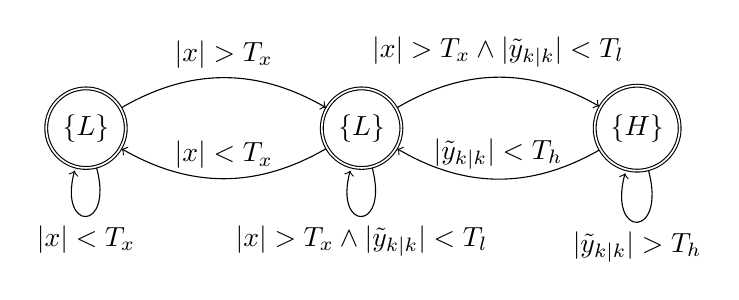
\begin{tikzpicture}[node distance=3.5cm,auto]
            \node (A) [state, accepting] {$\{L\}$};
            \node (B) [state, accepting] [right of=A] {$\{L\}$};
            \node (C) [state, accepting] [right of=B] {$\{H\}$};
            
            \path[->] (A) edge [loop below] node {$|x| < T_x$} (A);
            \path[->] (A) edge [bend left] node {$|x| > T_x$} (B);
            \path[->] (B) edge [bend left, above] node {$|x| < T_x$} (A);
            \path[->] (B) edge [loop below] node {$|x| > T_x \wedge |\tilde{y}_{k|k}| < T_l$} (B);
            
            \path[->] (B) edge [bend left] node {$|x| > T_x \wedge |\tilde{y}_{k|k}| < T_l$} (C);
            \path[->] (C) edge [bend left, above] node {$ |\tilde{y}_{k|k}| < T_h$} (B);
            \path[->] (C) edge [loop below] node {$ |\tilde{y}_{k|k}| > T_h$} (C);
            %\path[->] (B) edge [bend left] node {$s_{0.7} \wedge est_1$} (A);
            \end{tikzpicture}
        }
        
        \\ 
        \multicolumn{2}{c}{\LARGE $A_{comp1}$}\\[10pt]
        \hline
        
        % 4 state
        %TODO - Hodai say: this is non-deterministic automata for sipmlicity
        \multicolumn{2}{c}{
            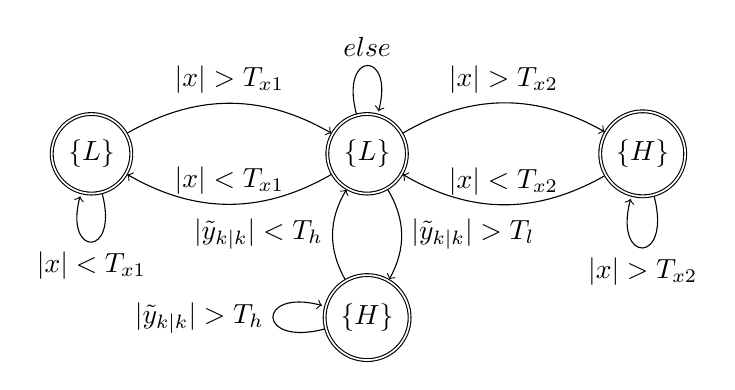
\begin{tikzpicture}[node distance=3.5cm,auto]
            \node (A) [state, accepting] {$\{L\}$};
            \node (B) [state, accepting] [right of=A] {$\{L\}$};
            \node (C) [state, accepting] [right of=B] {$\{H\}$};
            \node (D) [state, accepting] [below=1cm of B] {$\{H\}$};
            
            \path[->] (A) edge [loop below] node {$|x| < T_{x1}$} (A);
            \path[->] (A) edge [bend left] node {$|x| > T_{x1}$} (B);
            \path[->] (B) edge [bend left, above] node {$|x| < T_{x1}$} (A);
            
            \path[->] (B) edge [loop above] node {$else$} (B);
            
            \path[->] (B) edge [bend left] node {$|x| > T_{x2}$} (C);
            \path[->] (C) edge [bend left, above] node {$|x| < T_{x2}$} (B);
            \path[->] (C) edge [loop below] node {$|x| > T_{x2}$} (C);
            
            \path[->] (B) edge [bend left] node {$|\tilde{y}_{k|k}| > T_l$} (D);
            \path[->] (D) edge [bend left] node {$|\tilde{y}_{k|k}| < T_h$} (B);
            \path[->] (D) edge [loop left] node {$|\tilde{y}_{k|k}| > T_h$} (D);
            \end{tikzpicture}
        }
        \\
        \multicolumn{2}{c}{\LARGE $A_{comp2}$}\\
        
        
    \end{tabular}
    
    \caption{The main Automata we used for the requirements specifications in the experiments. 
        $A_{err}$ uses the \textit{measurement post-fit residual} ($\tilde{y}_{k|k}$), if $|\tilde{y}_{k|k}|$ is too small then the next iteration will use small resolution image ($L$), and if it is too large the high resolution will be used, $T_l$ and $T_h$ are the transition thresholds.
        $A_x$ operates similar to $A_{err}$, only it uses the current position (the $x$ part of $\hat{x}_{k|k}$) instead of $\tilde{y}_{k|k}$, with the threshold $T_x$.
        $A_{comp1}$ and $A_{comp2}$ area composition of the ideas in $A_{err}$ and in $A_x$.}
    
    \label{fig:test_automata}
\end{figure}

%%%%%%%%%%% results %%%%%%%%%%%%%
\section{Results}
\label{sec:results}

Table~\ref{tab:results} summarizes the result of the flight experiments made using the specification automata described in Section~\ref{sec:Analysis}.
The first column ``\% CPU'' represents processing time usage by the image processing task.
The second column ``$mean(|$x$|)$'' is the average distance of the drone from the origin in centimeters.
All the statistics shown in the table are from real indoor experiment flights. Each experiment consists of a flight (between one and two minutes) recorded using an \textit{OptiTrack} system (see Section~\ref{sec:Experiment setup}) and data from the software itself.

We see that, using reactive scheduling methods, we can adjust the trade-off between performance and CPU usage. As expected, if we use \textbf{only high} resolution mode we get the best performance but need much \%CPU. On the other hand, the \textbf{only low} resolution mode barely use the processor but the performance are low and unsatisfying for indoor flights.

In Table~\ref{tab:results}, automata number 3,4 and 5 are the implementation of $A_{x}$ automaton as describe in Section~\ref{sec:Analysis} with the threshold values of 10, 20 and 30cm respectively.
Those schedulers demonstrate that even a simple scheduling scheme, that schedules the expensive image processing task only when it is most needed, improves the performance. Scheduler number 3 achieves almost the same performance as the only high resolution scheduler but saves half of the CPU time. Scheduler automata 4 and 5 provide different trade-offs.

The $A_{err}$ automaton (shown in Figure~\ref{fig:test_automata}), which bases its transitions on $\tilde{y}_{k|k}$, appears to be even more effective.
We tested this automaton with ($T_l=10 , T_h=20$) and ($T_l=10 , T_h=15$) thresholds as shown by schedulers 6 and 7 respectively in Table~\ref{tab:results}.
They are using even less CPU time but still achieve fairly impressive performance.
The more complex schedulers contribute even more to the performance and utilization. Scheduler $A_{comp1}$ for example achieves a little better resource utilization.
The methodology we are proposing is to tune the thresholds and to enrich the automata, as we did, until satisfactory CPU utilization and performance are achieved.

Another advantage we achieved using the dynamic schedulers, beyond allowing better performance to computation load balance, is reactiveness. The  scheduling scheme we are proposing allows the system to adapts itself to changes in environmental conditions, demonstrated as follows.
We experimented in exposing the flying drone to time-varying wind conditions. 
Specifically, we created artificial wind by turning  on a fan while the drone was flying. The scheduler was the $A_{err}$ automaton with the thresholds $T_l=10$ and $T_h=15$ (number~7 in Table~\ref{tab:results}).
Figure~\ref{fig:windPlot} shows data collected in one of the flights with the CPU usage and the displacement of the drone along the flight. The first part of the flight, colored in blue, is indoor flight without any external wind. The second part, colored in red, is a flight with the disturbance caused by the wind of the fan. We can clearly see increasing CPU usage when there is wind. We can also see that the wind does not affect the displacement, as the increased accuracy of the sensor compensates for it. The mean displacement ($mean(|x|$) in this experiment was 11.8cm which is very close to the displacement without the wind, and the average CPU usage increased to  13.2\% from 11.7\%. This experiment further demonstrates our idea: resources can be allocated only when needed.

\begin{table} %[htbp]
    \caption{Test Results}
    \begin{center}
        \begin{tabular}{c  | m{10em} |  m{4em} | m{5em} }
            %\begin{tabular}{m{6em} |  c c c}
            \hline
            %\textbf{Observer}& CPU usage (\%)  & Mean displacement ($x$ axis) & Max displacement ($x$ axis)\\
            & \textbf{Schedule}& \textbf{\% CPU}  & \textbf{mean($|x|$) (cm)} \\
            \hline
            (1)& Only High & 30.9\% & 9.5\\
            \hline
            (2)& Only Low & 2.1\% & 30.0\\
            \hline
            (3)& $A_{x}$  ($T_x=10$) & 16.6\% & 10.9\\
            \hline
            (4)& $A_{x}$  ($T_x=20$)  & 14.0\% & 14.1  \\
            \hline
            (5)& $A_{x}$  ($T_x=30$)  & 8.9\% & 17.4  \\
            \hline
            (6)& $A_{err}$ \newline ($T_l=10 , T_h=20$) & 10.3\% & 14.9 \\
            \hline
            (7)& $A_{err}$ \newline ($T_l=10 , T_h=15$) & 11.7\% & 11.3 \\
            \hline
            (8)& $A_{comp1}$ \newline ($T_x=10$ , $T_l=10$ , $T_h=15$)  & 8.8\% & 12.9 \\
            \hline
            (9)& $A_{comp2}$ \newline ($T_{x1}=10$ , $T_{x2}=30$ , $T_l=10$ , $T_h=15$)   & 10.4\% & 12.7 \\
            \hline
            
        \end{tabular}
        \label{tab:results}
    \end{center}
\end{table}

\begin{figure} %[htbp]
    \centerline{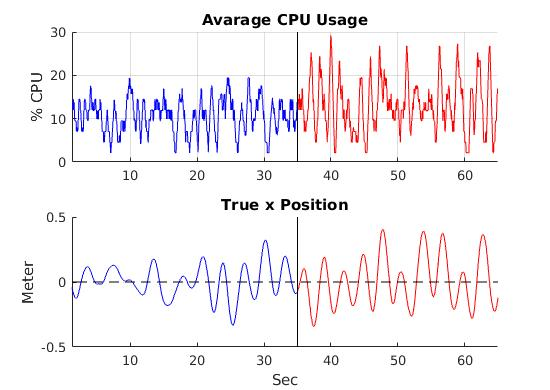
\includegraphics[width=100mm]{windPlot15.jpg}}
    \caption{This figure demonstrates how the reactive scheduler adapt to the environment changes, in particular, to change of the wind. The upper part shows the average CPU usage during the flight, and the bottom is the true position at the same time. The first part of the flight (the left Blue graph) is without any external wind and in the rest of the flight (right red graph)  the drone was exposed to artificial wind (using a fan). Note that when the drone is exposed to wind it uses more CPU to compensate for the disturbance.}
    \label{fig:windPlot}
\end{figure}

\section{Experiment Setup}
\label{sec:Experiment setup}

\begin{figure} %[htbp]
    \centerline{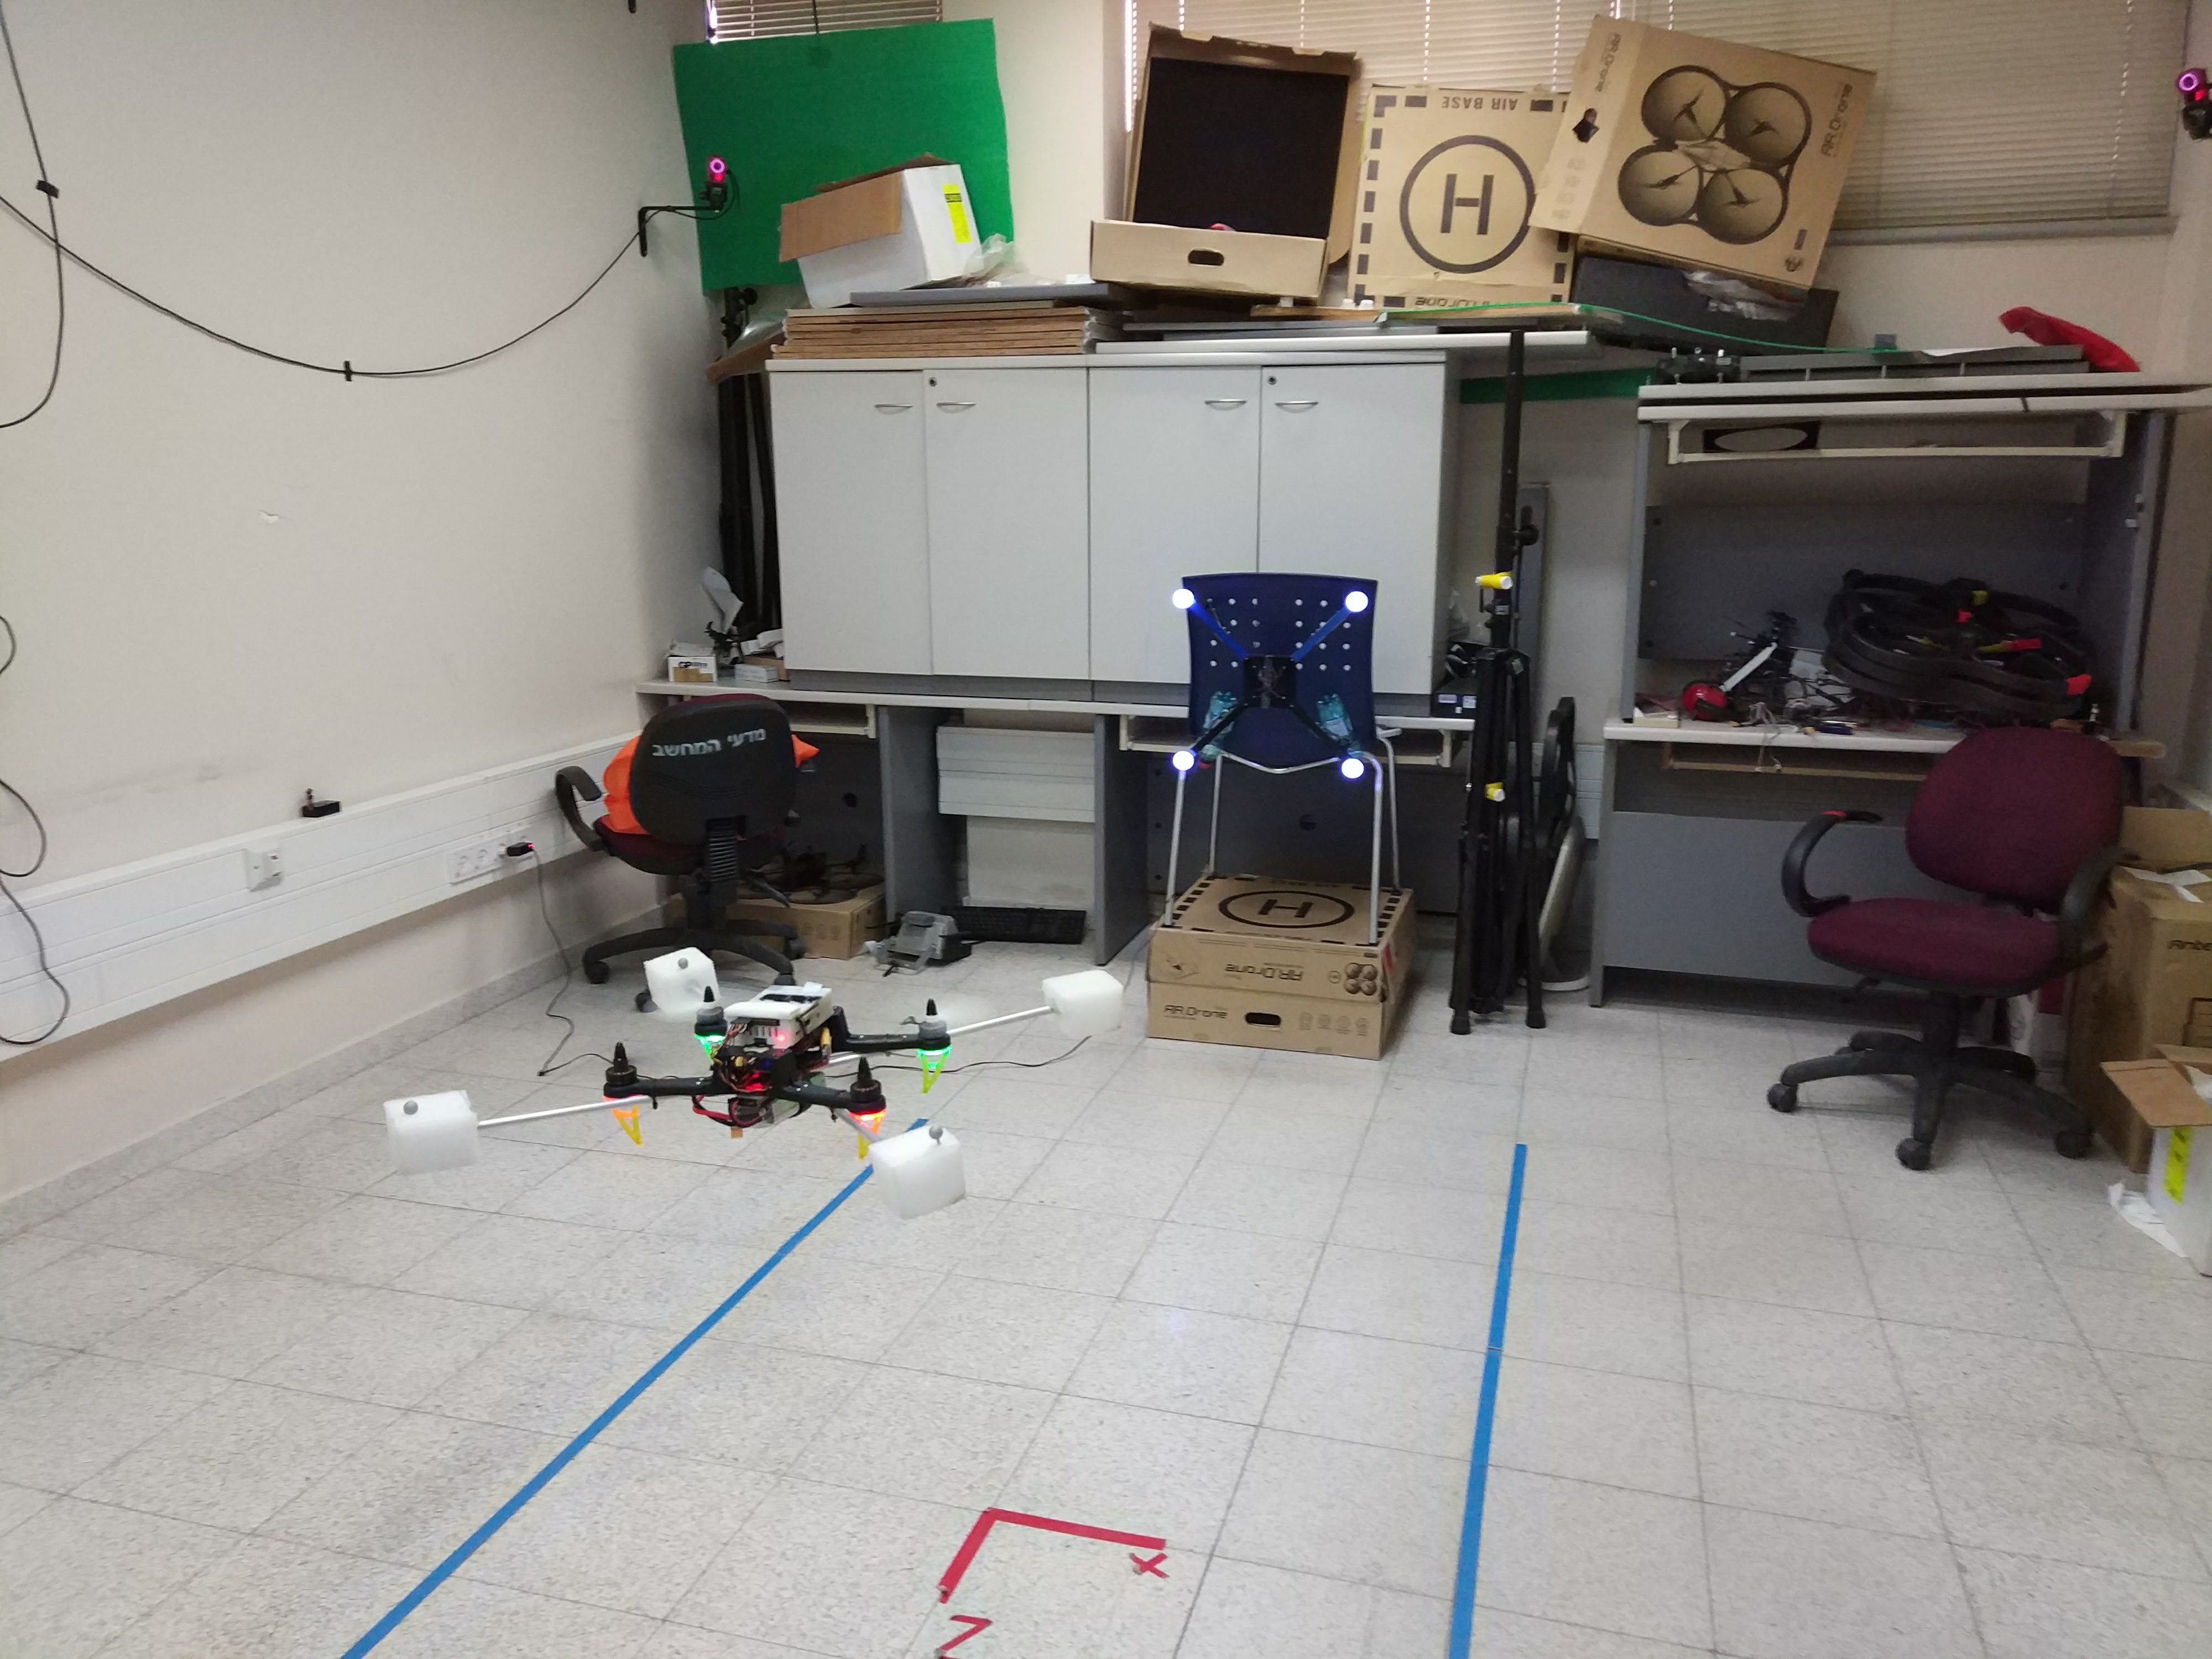
\includegraphics[width=100mm]{hover_in_lab.jpg}}
    \caption{This figure shows the drone hovering in front of the window during one of the experiments in our lab, window in the test is just 4 light balls.}
    \label{fig:hover_in_lab}
\end{figure}

\subsection{Hardware - the Quad-Rotor}
\label{sec:Experiment setup-HW}
% the hardware

In order to perform the experiments we used an of-the-shelf quadrotor shown in Figure~\ref{fig:hover_in_lab} with improved flight controlle: a \textit{raspberry-pi}, a single-board computer~\cite{raspberry}, with the \textit{navio2}~\cite{navio} shield.
\textit{Navio2} is extension board (shield) for the \textit{Raspberry pi} platform, it provides the nessesary interfaces such as remote control inputs and motors output, and it is equipped with on-board Micro Electro-Mechanical System (MEMS) sensors, such as rate gyros and accelerometers.
We implemented the controllers and the schedulers as libraries for the ArduPilot Mega (APM) autopilot software~\cite{APM}.

\subsection{Vision Based Sensor}
\label{sec:Experiment setup-cam}
% PiCam and drivers
As explained in Section~\ref{sec:caseStudy} we use vision-based sensor for identify the window.
For this task we used the standard raspberry-pi camera module (V1) (see~\url{www.raspberrypi.org/documentation/hardware/camera/}) mounted in the front of the drone
This camera can take pictures in different resolutions and at different frame rate.
The controller software implemented in c++ therefore we initially use the most common used driver for C++ called  \textit{RaspiCam} (see~\url{www.uco.es/investiga/grupos/ava/node/40}.
RaspiCam have two main difficulties for us:
\begin{enumerate}
    \item The raspberry-pi camera take a picture in a constant pre-define frame rate~\footnote{The constant pre-define frame rate is only wen using ``vid'' mod which allows fast frame rate}, this mean that if we want to grab an image the driver (RaspiCam) will wait till the next frame is taking. This approach is not appropriate for real-time system.
    \item As describe in Section~\ref{sec:caseStudy} we need to switch image resolution during the flight many times, raspberry-pi camera resolution is defined only at initialization, therefore changing resolution of the camera results in significant delay till the camera is ready at the new resolution.
\end{enumerate} 

The first difficulty has solved by modifying RaspiCam driver, we add to RaspiCam the ability to notify the client when the next frame is ready, this way whenever a new frame is taken the callback function is called.
We also add this modification to the official RaspiCam code that is maintained in~\url{github.com/cedricve/raspicam}.

In order to overcome the second difficulty we try to take pictures at the high resolution and then resize by software (using OpenCV) to the desire resolution, this solution still add undesirable delay for each frame that is taking.
At the end, we create a new camera driver based on the work of Chris Cummings at~\url{robotblogging.blogspot.co.il/2013/10/an-efficient-and-simple-c-api-for.html}.
In this driver we use the internal GPU hardware of the Raspberry-py in order to resize the frame by hardware.
Using the ARM side libraries \textit{userland}~\url{https://github.com/raspberrypi/userland} we construct a up to 4 video ports each one from different resolution resizer all connected to the camera port (see Figure~\ref{fig:resize_ports}), now each time we want to take image we can choose the image resolution by retrieving the image from the corresponded port.

\begin{figure} %[htbp]
    \centering
    
    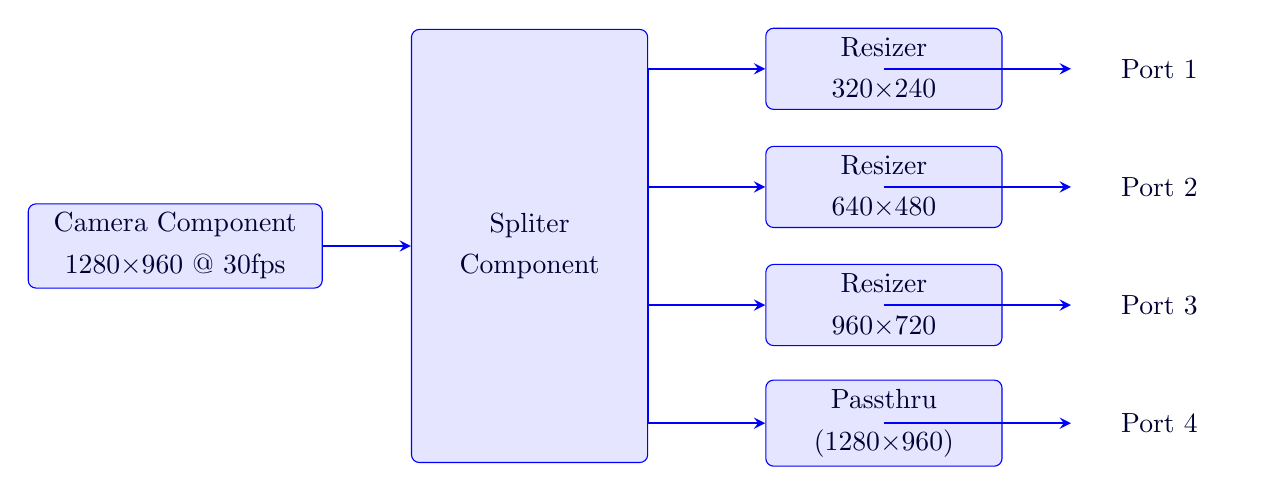
\begin{tikzpicture}[node distance=4.5cm]
        \node (cam) [recNodeB, text width=3.5cm] {Camera Component 1280$\times$960 @ 30fps};
        \node (sp) [recNodeB, text width=2cm, right of=cam, minimum height=5.5cm] {Spliter Component};
        \node (r1) [recNodeB, text width=2cm, right of=sp, yshift=2.25cm] {Resizer 320$\times$240 };
        \node (r2) [recNodeB, text width=2cm, right of=sp, yshift=0.75cm] {Resizer 640$\times$480};
        \node (r3) [recNodeB, text width=2cm, right of=sp, yshift=-0.75cm] {Resizer 960$\times$720};
        \node (r4) [recNodeB, text width=2cm, right of=sp, yshift=-2.25cm] {Passthru (1280$\times$960)};
        
        \draw [arrowB] (cam) -- node[above] {} (sp);
        \draw [arrowB] (sp.east) |- node[] {  } (r1.west);
        \draw [arrowB] (sp.east) |- node[] {  } (r2.west);
        \draw [arrowB] (sp.east) |- node[] {  } (r3.west);
        \draw [arrowB] (sp.east) |- node[] {  } (r4.west);
                
        \node (p1) [eNode, text width=2cm, right of=r1, xshift=-1cm] {Port 1};
        \node (p2) [eNode, text width=2cm, right of=r2, xshift=-1cm] {Port 2};
        \node (p3) [eNode, text width=2cm, right of=r3, xshift=-1cm] {Port 3};
        \node (p4) [eNode, text width=2cm, right of=r4, xshift=-1cm] {Port 4};
        
        \draw [arrowB] (r1) |- node[] {  } (p1);
        \draw [arrowB] (r2) |- node[] {  } (p2);
        \draw [arrowB] (r3) |- node[] {  } (p3);
        \draw [arrowB] (r4) |- node[] {  } (p4);
        
    \end{tikzpicture}
    
    \caption{This figure present the graphics processing unit (GPU) configuration we used for image resizing.}
    \label{fig:resize_ports}
\end{figure}

%vision algo
In the case-study, shown in Section~\ref{sec:caseStudy}, we always use the camera at 30 frames per second.
In order to simplify the image processing algorithm, we marked the four corners of the window with four illuminated balls (see Figure~\ref{fig:window_lights}). This allowed us to apply a simple minded corner detection algorithm: 
look for a blob of burned pixels and calculate the ``center of mass'' of all those pixels as a window corner. Higher resolution give us a more accurate measurement of corner ``center of mass'' but require more processing time.

\begin{figure} %[htbp]
    \centerline{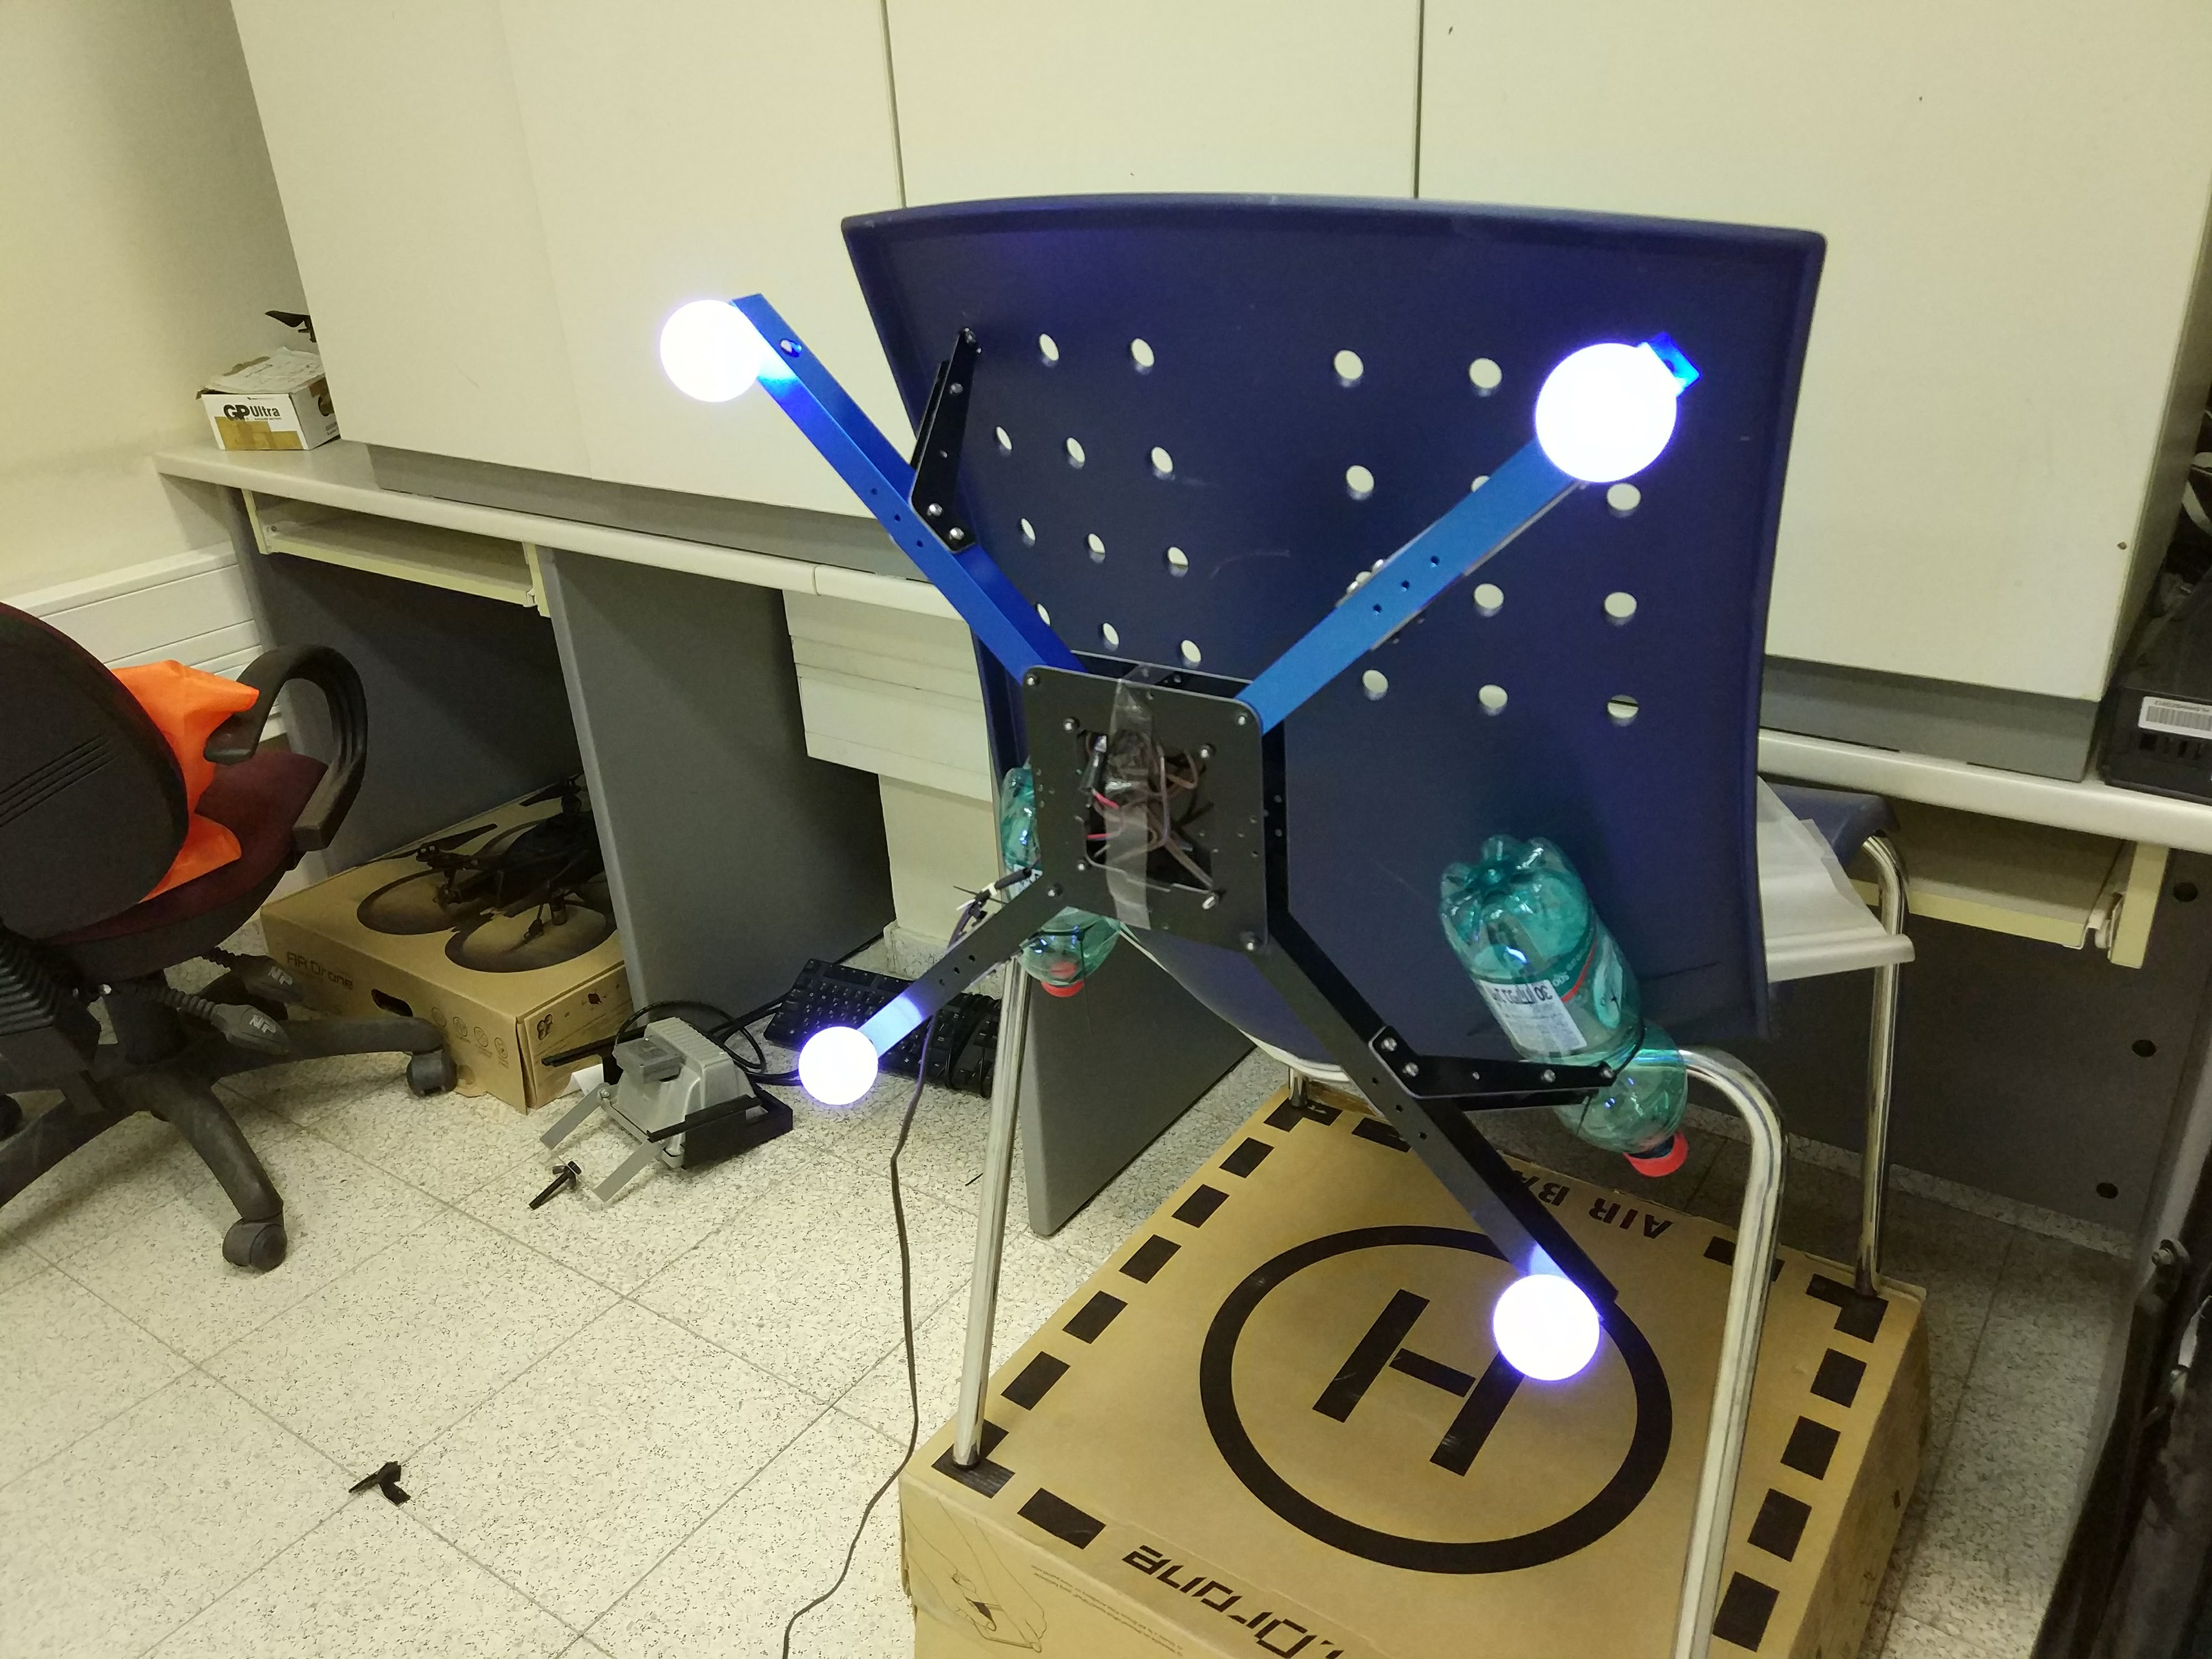
\includegraphics[width=70mm]{window_lights.jpg}}
    \caption{This figure shows the four light balls we used to represent the window during the experiment.}
    \label{fig:window_lights}
\end{figure}

\commentOut{
\subsubsection{Vision based Autonomous In-Door Flying}
%Anitime reserch of zilbershtain (\cite{Shlomo})
%contract based
%http://ardupilot.org/copter/docs/common-mouse-based-optical-flow-sensor-adns3080.html

\textit{Computer~Vision~Based~Sensor} is the module that is responsible for taking a picture or a series of pictures and produce measurements of quantities such as speed and position relative to the environment.
In our research we will use the \textit{Computer~Vision} in order to detect two dimensional movement in the camera surface (i.e., the drone speed).
There are many such algorithms (called optical flow) differing in running times and in accuracy. Usually more invested time leads to more accuracy.

In our case we need to be able to control the \textit{Computer~Vision} running time and to have some good knowledge of the solution accuracy in order to achieve optimal state estimation (see Section~\ref{sec:estimator}).
We assume that the \textit{Computer~Vision} error is distributed normally, and we will use the error variance as a measure of accuracy. 
We believe that this is a reasonable assumption because the estimated speed is usually computed as the avarage of of many independent random variables, as follows. Optic flow algorithms usually go by identifying similar regions in consecutive pictures and then averaging the distances that each feature ``traveled''. Assuming that the error in measurement of each feature is independent of the other errors, we get that the total error is the average of independent random variables. Then, by the law of large numbers, we get that the error should have a normal distribution. We will validate this assumption by experimentation with different parameters of different algorithms.

%TODO - reed a litle the article (\cite{UPenn-Pant}) and re-write the next.
%TODO - check if Anitime reserch (\cite{Shlomo}) can fit here.
%TODO - Make sure that we use the terms contract-base and any-time correctly
In order to control the running time, we will use anytime based algorithms~\cite{Shlomo} and will mainly concentrate on ``contract based" vision algorithms proposed by Pant~\cite{UPenn-Pant}.
This type of algorithms run until we stop them, and when we stop them they will provide a solution with accuracy that is a monotonic function of the amount of time it was running. That way we can control the solution accuracy by controlling the running time.
In our implementation, in order to lower the complexity, we will pre-define few specific ``operation modes" of the \textit{Computer~Vision} task, that differ by their running time and they are identified by a pair $\langle RunTime, Variance \rangle$ where $Variance$ is the error variance of running time $RunTime$.
}

\subsection{Reference Measurement with OptiTrack System}
%OptiTrack
In order to evaluate the performance, we needed to know the accurate position of the drone during the flight. For this purpose, we used the \textit{OptiTrack} (\url{optitrack.com}) system 
consisting of an array of high-speed tracking cameras that provide low latency and high accuracy position and attitude tracking of the drone. The data from \textit{OptiTrack} system is sent over the client-server data streaming protocol \textit{NatNet}.
For best synchronization, we create a NatNet client library inside the APM code. This library allows the controller check anytime for the current state and log that information in parallel to the other controller parameters.
We also use the OptiTrack information in early stages of the research as the feedback of the controller before we use the camera .

\section{Scheduler Interface}
\label{sec:scheduler}

The most common communication interface between scheduler and embedded real-time component, is by specify a period, sometimes along with a deadline, which gives the frequency at which the component must be executed.
The only requirement in those type of systems is that if the component is always executed exactly within the designed frequency (period), then the control objectives (e.g. stability) are met.
%not directly in this article
Specifying resource requirements using periods has advantages due to simplicity and analyzability, but has limited expressiveness, as elaborated in~\cite{RTComposer}. 
%For example, a specification such as “execute the component every 5ms” does not say whether the scheduler should or should not execute it more frequently if enough computing resources are available, and if a component has multiple, say, for different control tasks, each needing a different period, the requirement cannot be naturally captured by a single period.

In Section~\ref{sec:architecture} we have suggested to use automata for describe the component specification for the scheduler. In this section we elaborate the technical details of the specification automata.

In our framework, similarly to most traditional real time systems, the resource is allocated in discrete \textit{time slots} of fixed duration in the style of time-triggered architecture~\cite{RTComposer}.
A typical cyber-physical control system have multiple tasks that need to be done in order to control the system.
Each task is performed by one or more subroutines (code functions).
We suggest designing control system in the \textit{component} level, where each component is corresponding a specific task in the system, it consists of all the subroutines of the task, along with a \buchi game specify how the task subroutines should be executed.

\begin{dfn}
    A component is a pair $\langle T,G\rangle$ where $T$ is a set of subroutines (representing, e.g., procedures of a class in C++) and $G=\langle A,\langle P_{schd}, P_{env}\rangle \rangle$ is a generalized B{\"u}chi game (GNBG), over a generalized \buchi automaton $A= \langle Q,\Sigma,\Delta,q_0,\mathcal{F} \rangle $ (see Section~\ref{sec:GNBG}), such that:
    \begin{enumerate}
        \item The \textit{alphabet} is $\Sigma = 2^{T} \cup \R^n$ where $n$ is the number of scheduler feedback variables in the system (real numbers that the scheduler can base its decision on).
        \item 
        Alternating turns with different parts of the alphabet:
       	The transitions of $A$ are of the form: $s_{schd} \xrightarrow[]{\sigma_{T}} s_{env}$ where $s_{schd} \in P_{schd}, s_{env} \in P_{env},$ and $\sigma_{T} \subseteq T$ (called  ``scheduler'' transitions ),  or of the form $s_{env} \xrightarrow[]{\sigma_{e}} s_{schd}$, where $s_{schd} \in P_{schd}, s_{env} \in P_{env}$, and $\sigma_{e} \in \R^n$ (called ``environment'' transitions).
        \item The environment plays first: $q_0 \in P_{env}$.
    \end{enumerate}
\end{dfn}

The \buchi game $G=\langle A,\langle P_{schd}, P_{env}\rangle \rangle$, of a component, is a scheduler-against-environment game, it is represents the interaction of the controller and the environment in the real world.
The game goes as follows: before every time slot the environment player ($P_{env}$) play first and take the transition $s_{env} \xrightarrow[]{\sigma_{\vec{y}}} s_{schd}$ such that $\vec{y} \in \R^n$ was the observation values at the beginning of this slot.
Then the scheduler need to choose a transition $s_{schd} \xrightarrow[]{\sigma_{T'}} s_{env}'$, and then execute all the tasks in $\sigma_{T'}$.
The environment transition represent the evolution of the system state caused by the actuators and the environment of previous time step, and then the scheduler react to state evolution by the schedule transition.
This simultaneous walk over the game automata $A$ create
The scheduler goal is to pass infinitely many times in acceptance state during the execution.
In other words, if the world, $\omega = \vec{y}_1 , T_1, \vec{y}_2, \dots $, created by this simultaneous walk over the game automata $A$ is accepting world, $\omega \in \mathcal{L}_{\omega}(A)$.
Note, the scheduler feedback variable (or observations) is a vector $\vec{y} \in \R^n$ that may includes state variables and internal variable of the components.

An example of a vision based sensor component of a robot is demonstrated in Figure~\ref{fig:exampleGame}. 
The component estimates the robot position using a camera. It has two operation modes: high (H) or low (L) accuracy.
The variable $y$ is the estimated position, in this example the component requirement is to ensure that $y$ never exceeds one (in position $y=1$ there is a cliff). \todo{I don't know if this example is helping or not}

\begin{figure} [h]
    \centerline{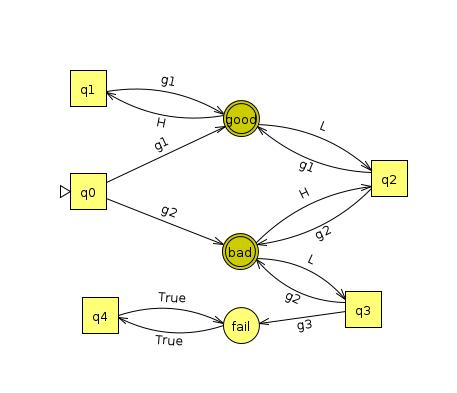
\includegraphics[width=100mm]{gameExample.jpg}}
    \caption{Example of a game for vision based sensor component of a robot.
        The robot must maintain position of $y \le 1$ where $H$ is high accuracy and $L$ is low accuracy position measuring tasks, and
        $g1$ refer to $y \le 0.5$, $g2$ refer to $0.5 < y \le 1$ and $g3$ refer to $1 < y$ }
    \label{fig:exampleGame}
\end{figure}

%\subsection{Component Games Composition}
As we said a typical system composed of multiple components that need to be executed simultaneously by the same processor.
Each component have its own game (its own requirements), therefore we will construct a composed component that correspond to all the system components together, then the scheduler have only one component, with only one game to win for scheduling all the components.
Let's define composition of the components, that preservative the logic and correction of its composed components.

\begin{dfn}
    The composition of the components $C_1=\langle T_1, \langle A_1, \langle P_{schd}^1, P_{env}^1\rangle\rangle\rangle$ and $C_2=\langle T_2, \langle A_2, \langle P_{schd}^2, P_{env}^2\rangle\rangle\rangle$ is the component $C_c = C_1 \times C_2 = \langle T_1 \cup T_2, \langle A_c, \langle P_{schd}^1 \times P_{schd}^2, P_{env}^1 \times P_{env}^2 \rangle\rangle\rangle$ where $A_c= \langle Q_1 \times Q_2,(T_1 \cup T_2) \times \R^n,\Delta_c,Q_0^1 \times Q_0^2,\mathcal{F}_1 \cup \mathcal{F}_2 \rangle$ is a product of $C_1$ and $C_2$ and 
    \begin{enumerate}
        \item Environment transitions: $\forall y \in \R^n, s_1 , s_1' \in Q_1, s_2 , s_2' \in Q_2$:
        $\langle s_{1} s_2 \rangle \xrightarrow[]{y} \langle s_{1}' s_2' \rangle \in \Delta_c$
        if and only if 
        $s_{1} \xrightarrow[]{y} s_{1}' \in \Delta_1$ and $s_{2} \xrightarrow[]{y} s_{2}' \in \Delta_2$.
        \item Scheduler transitions: $\forall T_1' \subseteq T_1,T_2' \subseteq T_2$ , $s_1 , s_1' \in Q_1, s_2 , s_2' \in Q_2$:
        $\langle s_{1} s_2 \rangle \xrightarrow[]{T_1' \cup T_2'} \langle s_{1}' s_2' \rangle \in \Delta_c$
        if and only if         
        $s_{1} \xrightarrow[]{T_1'} s_{1}' \in \Delta_1$ and $s_{2} \xrightarrow[]{T_2'} s_{2}' \in \Delta_2$.
    \end{enumerate}
\end{dfn}

Note: components composition is defined for compose two components, but we can compose all the system component, $C_1 , ... , C_m$, one by one: $C_c = (\cdots((C_1 \times C_2) \times C_3 ) \times \cdots \times C_m)$.

%\subsection{Add Resources Limitation}
In addition to the component requirements (requirements from control objective) we also have resources requirements, we have limited resources (limited CPU abilities) that need to be taking in account.
Resources requirements are reflected as limited time slot capacity, each subroutine (procedure) take some time to perform but the slot is limited in time.
For example, two subroutines $t_1$ and $t_2$ that require 1.5 millisecond each to execute, cannot be executed in 2 millisecond time slot.
We will enforce the slot size with a special and simple component $C_{reasource}$ that can be generated automatically as follows:
assuming we know the maximum duration of each subroutine of the components in the system (it can be result of analyzing, testing, or manually pre-defined) we construct component with the tasks set $T$ that is union of all the subroutines in the system, and the game ($G_{reasource}$) is as demonstrate in Figure~\ref{fig:C_reasource} with one state for environment player (square state) and one for the scheduler (circle state), the environment have no limitations but the scheduler can execute only set of tasks that not exceeds the time slot.

\begin{figure} [h]
    \centerline{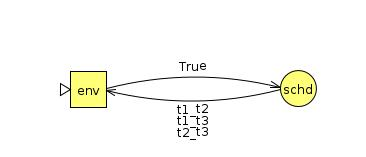
\includegraphics[width=80mm]{reasourceGame.jpg}}
    %\subfile{./goal/reasourceGame.tex}
    \caption{Example of a game for resource component that do not allows to exceed a time slot. 
        In this example $T = \left\{ t_1 , t_2 , t_3 \right\}$, the execution time of each task $t_i$ is half of a single time slot, therefore it is not possible to execute more than two tasks at the same time slot, but there is no limitation on the environment ($\vec{y}$).
        Square state is an environment player state and round state belong to the scheduler.  }
    \label{fig:C_reasource}
\end{figure}

Finally, the resource component is composed with all the rest components of the system resoult in the schedule component $C_s = C_{reasource} \times C_c$.

%\subsection{Wining the Game - Find the Strategy}
The component $C_s$ aggregates all the system constrains, in order to successfully schedule the system, we need to find a ``wining'' strategy $A_{strategy} \in NBA$ for the scheduler.
$A_{strategy}$ is in fact, a reduction of the game automaton $A_s = \langle Q_s ,\Sigma,\Delta_s, Q_0, \mathcal{F}_s \rangle$ of $C_s$. It is contained all the environment transitions in $A_s$, but only the scheduler transitions that allays can lead to a winning of the scheduler player, that is, runs that we visit infinitely times a state of every color $F' \in \mathcal{F}_s$.
Example of such strategy is shown in Figure~\ref{fig:exampleGameStrategy}, the blue partial automaton is the scheduler wining strategy for the game presented in Figure~\ref{fig:exampleGame} discussed before.
We call this winning strategy guarded automaton \todo{we can add here reference to the simpler guarded automata presented in the previews sections}.

\begin{figure}[h]
    \centerline{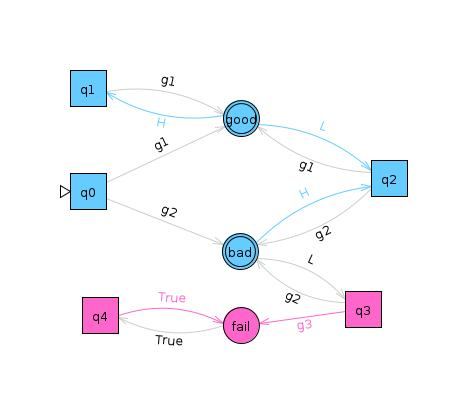
\includegraphics[width=100mm]{gameExampleSolved.jpg}}
    \caption{A strategy solution for the game presented in Figure~\ref{fig:exampleGame}.
        Blue states are all the states which the scheduler have a wining strategy from them, blue transitions are the needed scheduler reaction to win the game.
        Note: if the initial state is blue then the system is schedulable.}
    \label{fig:exampleGameStrategy}
\end{figure}










%TODO - continue here

\subsection{Execution of the scheduler}

Each time the system is executed the scheduler just walk through the strategy automaton $A_s$ as describe by the pseudo code~\ref{code:scheduler}. 
The time is divided into segments of equal length called ``time step''.
At the beginning of each time step the current automaton state is environment player state, so we pick the \todo{continue verbal explanation of the pseudo cod }

\begin{algorithm}[h]
    \caption{Scheduler run-time operation}
    \begin{algorithmic}[1]
        \Procedure{Schedule}{$A_s$} \Comment{schedule the system with strategy automaton $A_s$ }
            %\State \Call{Validate}{$A_s$} \Comment{validate that $A_s$ is wining strategy}
            \State $cur\_state \gets$ \Call{Initial}{$A_s$} \Comment{start with the initial state}
            
            \Statex
            \Loop 
                \State $\vec{y} \gets \Call{getStateVars}$
                
                \State $cur\_state \gets$ \Call{Next}{$cur\_state$ , $\vec{y}$} \Comment{take environment transition for $\vec{y}$ }
                \If {$cur\_state == None$}
                    \State Exit \Comment{unexpected $\vec{y}$ value, fail to proceed}
                \EndIf
                
                \Statex
                \State $\delta \gets$ \Call{getFirstTransition}{$cur\_state$} \Comment{take scheduler transition}
                \State $Tasks \gets$ \Call{tasks}{$\delta$}
                \State $cur\_state \gets$ \Call{toState}{$\delta$}
                
                \ForAll{ $t \in Tasks$} \Comment{execute all the tasks defined by the transition}
                    \State \Call{Execute} {$t$}
                \EndFor
                
                \Statex
                \State Wait till next time step
                
            \EndLoop
        \EndProcedure
    \end{algorithmic}
    \label{code:scheduler}
\end{algorithm}

\subsection{Correctness}

\begin{dfn}
    A component $C_i$ is ``complete'' if for each $t_1, \dots, t_m \subseteq T_i$, $\vec{y}_1, \dots , \vec{y}_m \in \R^n$ and $q_e \in P_{env}$ such that there is a path from $q_0$ to $q_e$ with the word $w= \vec{y}_1 , t_1 , \vec{y}_2 , t_2, \dots , \vec{y}_{m}, t_m$ we have that for each $\vec{y}_{m+1}$ that can be observed after any run of the system that corresponds to this word (i.e., a run where after each observation $\vec{y}_j$ we scheduled $t_j$) there is a transition from $q_e$ labeled with $\vec{y}_{m+1}$.
\end{dfn}

\begin{dfn}
    A component $C_i$ is well-formed if it is complete and if in  any execution whose observations and task schedules constitute a word $\omega \in \mathcal{L}(A_i)$, the component achieves its control objectives.
\end{dfn}

\begin{claim}
    \label{thm:valid_composition}
    If $C_1$ and $C_2$ are a well-formed components then their composition $C_c=C_1 \cdot C_2$ is also a well-formed component.
\end{claim}
\begin{proof}
    \begin{enumerate}
        \item $C_c$ is a component: trivial \todo{maybe just the transitions rule is not trivial}
        
        % all posible y
        \item $C_c$ is complete component: Assume that after we get to state $\langle q_1 , q_2 \rangle \in P_{env}^1 \times P_{env}^2$ we may observe $\vec{y}$, then because $C_1$ is complete there is a transition $q_1 \xrightarrow[]{\vec{y}} q_1'$ and same for $q_2 \xrightarrow[]{\vec{y}} q_2'$ in $C_2$, therefore by the composition definition $A_c$ contains the transition $\langle q_1 , q_2 \rangle \xrightarrow[]{\vec{y}} \langle q_1' , q_2' \rangle$
        
        \item $C_c$ satisfy its requirements: by composition definition the word $\omega= \vec{y}_1 , t_1 , \vec{y}_2 , t_2, ... \in \L(A_c)$ if and only if there exist words $\omega_1= \vec{y}_1 , t_1^1 , \vec{y}_2^1 , t_2, ... \in \L(A_1)$ and $\omega_2= \vec{y}_1 , t_1^2 , \vec{y}_2 , t_2^2, ... \in \L(A_2)$ such that $t_i = t_i^1 \cup t_i^2$. 
        Therefore, for each $\omega = \vec{y}_1 , t_1 , \vec{y}_2 , t_2, ... \in \L(A_c)$ a system execution that before each time slot $j$ observe $\vec{y}_j$ and then execute the tasks $t_i$ in that slot is in particular execute $t_i^1$ and because $\omega_1= \vec{y}_1 , t_1^1 , \vec{y}_2^1 , t_2, ... \in \L(A_1)$ satisfies $C_1$ requirements $\omega$ also satisfying $C_1$ requirements, similarly, $\omega$ also satisfying $C_2$, then $\omega$ is a system execution that satisfies the requirement from the component (for the system).
        
    \end{enumerate}
\end{proof}

\begin{dfn}
	A system is ``schedulable'' if for any possible behavior of the environment (measurements that it may produce) there is a way for the scheduler to assign tasks such that all components achieve their control objectives.
\end{dfn}

\begin{claim}
    If $C_1,\dots , C_m$ are a well-formed components and there is a wining strategy for the composed component $C_s=C_1 \times \cdots \times C_m \times C_ {resource}$, then the system defined by $C_s$ is schedulable.
\end{claim}
\begin{proof}
    First note that $C_reasource$ is valid component:
    The only environment state of $A_reasource$ accept all $\R^n$ for the observations therefore $C_reasource$ is complete, the only requirement from $C_reasource$ is that the time step is never exceeded it length, this is guarantied by the contraction of scheduler transitions then $C_reasource$ is also satisfy its requirement so $C_reasource$ is valid component.
    All components $C_1 , C_2 , .. , C_m$ and $C_reasource $ are valid components then by Claim~\ref{thm:valid_composition} $C_s $ is valid component.
    
    Assume there is a wining strategy for $C_s$ then the scheduler that random walk trough the wining strategy automaton, and operate as elaborate in Algorithm~\ref{code:scheduler} is:
    \begin{enumerate}
        \item Never get stuck: $C_s$ is complete so each environment state of $A_s$ have transition for any possible observation and any strategy of scheduler must keep all environment transitions therefore the execution never get stuck at environment state, and each scheduler state in the strategy have at least one outcome transition because if this is not the case then the strategy is not a wining strategy. 
        
        \item The component $C_{resource}$ game have only transitions with task sets that even at the worst case they never exceeds a single time step and $T_{resource}$ contains all the system components tasks, therefore, $C_s$ also do not contain tasks sets that exceeds a single time step, therefore a schedule of a longer tasks set is not possible in algorithm~\ref{code:scheduler}.
        
        \item Satisfy the system requirements: The component $C_s$ satisfy its requirements, and the random walk of algorithm~\ref{code:scheduler} is also constructing a word $\omega \in \L(C_s)$, therefore by the definition of component that "satisfy its requirement", algorithm~\ref{code:scheduler} satisfy all the components requirements.
    \end{enumerate}
\end{proof}

\begin{remark}
    The fact that a system is schedulable, is not necessarily implies the there is a wining strategy.
\end{remark}







%TODO - continue here!
%TODO - maybe here insert a reference to preveus "mode based" automata
%TODO - we can add demonstration of how to define periodic tasks with automata
\subsection{Few Words about Implementation}

% finite space by discretization of observations (Merav)
% game solver - GOAL

% preparation time vs run time












\commentOut{





\subsection{Automata Operation - Creating the Composed automaton }

In order to schedule the complete system, we need first to construct an automaton (called composed automaton) that represent the requirement of the entire system, and never exceed the time-slot.
The composed automaton, called $A_{cmp}$, is constructed at the initialization or compilation time as follows:
Assume we have $n$ guarded automatons $[A_1 .. A_n]$ over $m$ subroutines (tasks) in the system, then:
\begin{enumerate}
    \item Intersect all automata: $A_{int}= \cap_{i=1}^{n} A_i$
    \item Construct overflow protection automaton ($A_{nof}$) as demonstrate in Figure~\ref{fig:A_{nof}} where $\Sigma_{nof}$ is set of all the letters that do not exceed the time-slot
    \item Intersect with the overflow protection automaton: $A_{cmp} =  A_{nof} \cup A_{int}$
    \item Analyze $A_{cmp}$ for schedule-ability, emptiness, etc.
\end{enumerate}

% Prof that composed automaton represent the requirement of the entire system
\todo{fix the definition of tasks that can consist of many subroutines}
A short proof that $A_{cmp}$ we construct satisfy the requirement of the entire system:
By definition, the language $L(A_i)$ of $A_i$ contain all the schedules that satisfy the requirement of $t_i$ and only them.
The intersection language $L(A_{int})= \cap_{i=1}^{n} L(A_i) $ state that: 
(1) if $\omega_j$ is legal schedule for the entire system $\omega_j \in L(A_{int})$ then $\forall i \in [1..n] : \omega_j \in L(A_i)$ mean $\omega_j$ is a schedule that satisfy the requirements of all the tasks in the system,
and (2) if $\omega_j$ not satisfy some task $i$ requirements ($\exists i \in [1..n] : \omega_j \notin L(A_i) $) then $\omega_j \notin L(A_{int})$. 
Therefore, the intersection automaton $A_{int}$ contains all the schedules that satisfy the requirements of all the tasks and only them.

% eliminate exceeds words
The automaton $A_{int}$ may still contain schedule that exceeds the time slot, we need to make sure that the scheduler never exceeds a single time-slot size ($ts$), that is, $\forall \omega_j \in A_{int} : \forall \sigma_k \in \omega_j \text{~s.t.~} time( task(\sigma_k)) \le st $.
Let's define $\Sigma_{nof} \subseteq \Sigma$ as set of all the letters $\sigma \in \Sigma$ that their tasks group do not exceed the time-slot ($time( task(\sigma)) \le ts$), then $L((\Sigma_{nof})^\omega)$ contain all the schedules that never exceeds the time-slot, this language can be easy defined by the automaton $A_{nof}$ presented in Figure~\ref{fig:A_{nof}}. 
Therefore, the automaton $A_{cmp} =  A_{nof} \cup A_{int}$ define exactly all the schedules that satisfy the requirements of all the tasks and never exceeds the time-slot.

% Analisys
After we construct $A_{cmp}$ we need to analyze it, we need to make sure that the system is schedule-able, that is, the scheduler never got stuck in a state with no appropriate transition for the next iteration.
This can be verified in few different levels, for example an easy and conservative technique is to check formally that from every accessible state $q_i$ of $A_{cmp}$ ``OR'' operation of all it outgoing transitions is ``True'': $\vee_{(q_i, \left < t_j, c_j \right > , q_k)}  c_j = \text{true} $. 
In case that we have some assumptions about the system behavior, we can use that information to make more accurate analysis, for example, assuming after executing ``high quality'' mode of image processing always $|y-\hat{y}| < 0.5$, under that assumption we can conclude that schedule using the follows automaton never stack:
\todo{I think the example is meaningless without explanation}
\begin{center}
    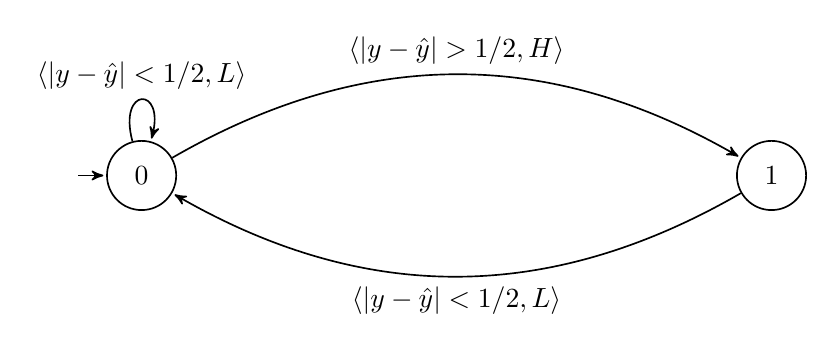
\begin{tikzpicture}[->,>=stealth',shorten >=1pt,auto,node distance=8cm, semithick]
    
    \node[initial,state] (A)                 {$0$};
    \node[state]         (B) [right of=A]    {$1$};
    
    \path (B) edge [bend left]             node {$\left < |y-\hat{y}|< 1/2 , L \right >$} (A);
%    (A) edge [loop below] node {$|y-\hat{y}|<1$} (A);
    
    \path (A) edge [bend left]             node {$\left < |y-\hat{y}| > 1/2 , H \right >$} (B);
    \path (A) edge [loop above] node {$\left < |y-\hat{y}| < 1/2 , L \right >$} (A);
    
    \end{tikzpicture}
\end{center}
} 

\commentOut{
\subsubsection{The Proposed Scheduling Methodology}
In this thesis we develop a new methodology for allocation resources. We focus on how should engineers describe the requirements of a real-time component.
To simplify, we will assume that the resource is allocated in discrete \textit{time slots} of fixed duration in the style of time-triggered architecture~\cite{RTComposer}.
%TODO - read again this section
%We will develop automata based (hybrid automata) methodologies and schedulers based on the work of Alur~\cite{RTComposer} and Bukra~\cite{Merav}, and will demonstrate with measurable data how they improve the performance of real flying drones (see Section~\ref{sec:results}).
The specification framework for resource requirements is based on \textit{Nondeterministic $\omega$-automata} (finite automata over infinite words)~\cite{???}.
Automata can be more expressive for describing specific requirements, and they are composable, i.e., it is easy to compose all the tasks requirements into an integrated automata, and its easy to analyze and manipulate using tools like GOAL~\cite{???}.


%TODO - what we do with $Acc$
Formally \textit{task specification automata} is defined, similarly to Nondeterministic $\omega$-automata, as tuple $A=(Q,\Sigma,\Delta,Q_0,Acc)$.
In our setting, the \textit{alphabet} of the automata is $\Sigma = T^2 \times C^2$ where 
$C$ is the set of Boolean conditions variables, will be describe later, and $T$ is the set of all tasks in the system.
Each infinite word ($\alpha \in \Sigma^\omega$) of the automata define a possible tasks scheduling over a fixed period (time slots), and the automata language define all the possible scheduling.
Now the scheduler only need to ``walk through'' the automata as follows, before every iteration (time slot) the scheduler choose state transition $(q_i , \{t_j , c_j\}, q_{i+1})$ from the current state $q_i$ to the state $q_{i+1}$


Let's define $s()$









%Hybrid automata is a variation of finite automata for real-valued continuously progressing words~\cite{hibrid-systems}.
In our setting, the automata define continuous (fixed period) operation modes, and the condition of mode changing.
The operation mode directly define a set of tasks that will be executed in the time slot (for example $s_{0.7}$ in Figure~\ref{fig:sched_sense_auto}).
We can stay at a single mode for some iterations, in this case the same tasks will be scheduled in each iteration. 
We can also take \textbf{discrete mode transition} in order to change operation mode after few iterations and schedule different set of tasks, for example, in Figure~\ref{fig:sched_sense_auto} the edge $(m_1,m_2)$ says that if the previous iteration mode was $m_1$ and $estVar < 0.7$ we can change the mode and schedule the set $\{s_{0.2}\}$ in the next iteration.

Each infinite path on the composed hybrid automata (not necessarily with infinitely many mode transitions) represents a schedule that satisfy all the tasks requirements. 
In this architecture the scheduler only need to ``walk through'' the composed automata, this is, of course, a fast and easy computational task. 
In order to assure that we do not exceed the time slot duration, each task will have pre-defined maximum duration time like ``deadline'' in the traditional architecture. Now we can verify that every possible scheduling step can execute within a single time slot, in other words, every mode of the composed automata can be executed in a single time slot, by simply summing the ``deadlines'' of all the tasks in the mode tasks set.
%we can summarize the total slot ``deadline'' as follows:\\
%$\forall mode~e ~~(\sum_{t \in Guard(e)} deadline(t) ) \leq slot~duration$ \\
If we find a mode that goes beyond the maximum duration we can remove it from the automata so we never exceed the time slot duration.


\begin{figure}[]
    \centering
    
    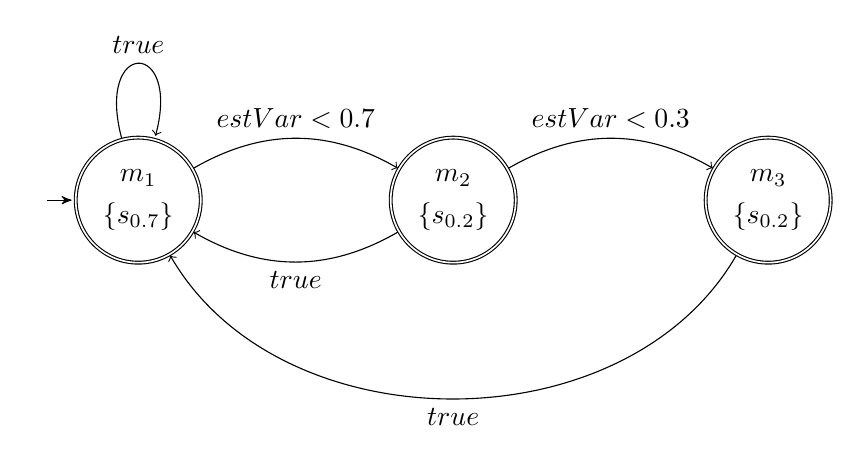
\begin{tikzpicture}[node distance=4cm, text centered, auto]
    \node (A) [state, accepting, text width=1cm, initial] {$m_1$ $\{s_{0.7}\}$};
    \node (B) [state, accepting, text width=1cm] [right of=A] {$m_2$ $\{s_{0.2}\}$};
    \node (C) [state, accepting, text width=1cm] [right of=B] {$m_3$ $\{s_{0.2}\}$};
    
    \path[->] (A) edge [loop above] node {$true$} (A);
    %\path[->] (A) edge [bend left] node {$\neg est_{bad} \wedge s_{0.2}$} (B);
    \path[->] (A) edge [bend left] node {$estVar < 0.7$} (B);
    \path[->] (B) edge [bend left] node {$true$} (A);
    %\path[->] (B) edge [loop above] node {$\neg var3$} (B);
    %\path[->] (B) edge [bend left] node {$est_{good} \wedge s_{0.2}$} (C);
    \path[->] (B) edge [bend left] node {$ estVar < 0.3$} (C);
    %\path[->] (C) edge [loop above] node {$var1$} (C);
    \path[->] (C) edge [bend left=60] node {$true$} (A);
    
    
    \end{tikzpicture}
    
    \caption{Example of guarded automata for our vision based sensor task, in this example the task has two operation modes, $\mathbf{s_{0.7}}$ which need 70\% of the time slot but is more accurate vision computation and $\mathbf{s_{0.2}}$ which is less accurate but faster (need only 20\% of the slot).
        The value of $estVar$ is $var(x-\tilde{x})$ of the previous iteration.
        Every time slot exactly one of the modes will be executed.
        \label{fig:sched_sense_auto}}
\end{figure}

\begin{figure}[]
    \centering
    
    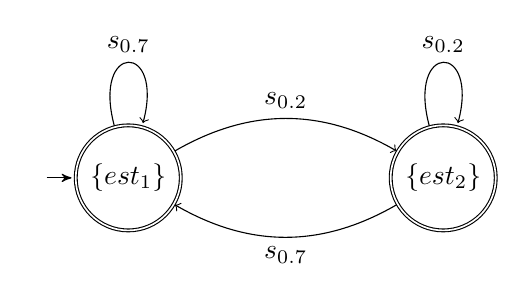
\begin{tikzpicture}[node distance=4cm,auto]
    \node (A) [state, accepting, initial] {$\{est_1\}$};
    \node (B) [state, accepting] [right of=A] {$\{est_2\}$};
    
    \path[->] (A) edge [loop above] node {$s_{0.7}$} (A);
    \path[->] (B) edge [bend left] node {$s_{0.7}$} (A);
    %\path[->] (A) edge [bend left] node {$s_{0.2} \wedge est_2$} (B);
    %\path[->] (B) edge [loop above] node {$s_{0.2} \wedge est_2$} (B);
    \path[->] (A) edge [bend left] node {$s_{0.2}$} (B);
    \path[->] (B) edge [loop above] node {$s_{0.2}$} (B);
    %\path[->] (B) edge [bend left] node {$s_{0.7} \wedge est_1$} (A);
    
    \end{tikzpicture}
    
    \caption{Example of guarded automata for our state estimator, in this example the estimator has two operation modes, $\mathbf{est_1}$ correspond to $\mathbf{s_{0.7}}$ and $\mathbf{est_2}$ correspond to $\mathbf{s_{0.2}}$~(see Figure \ref{fig:sched_sense_auto}).
        \label{fig:sched_estimator_auto}}
\end{figure}

Let us demonstrate the proposed automata based interface using the system depicted in Figure~\ref{fig:hybrid_loop}.
Assume we have two operation modes of the vision based sensor: (1) $s_{0.7}$ a very accurate operation mode that takes 70\% of the time slot to execute, that is of course a significant amount of time, and (2) $s_{0.2}$ a less accurate operation mode but takes only 20\% of the slot.
In each time slot we can execute one of them and get the sensing process done, but if we use only $s_{0.7}$ every time slot we may not have enough time to execute all the tasks. On the other hand, if we use only $s_{0.2}$ we will have inferior estimates.
Figure~\ref{fig:sched_sense_auto} shows an example of a guarded automata that guides the schedule. With this automata we can express rich specifications. 
In this example, execute $s_{0.7}$ is always allowed but if we need faster sensing we can use $s_{0.2}$ but only once in a row if the estimation error is not extremely bad~(if~$var(x-\tilde{x}) < 0.7$), or even twice in a row if the estimation error is good~(if~$var(x-\tilde{x}) < 0.3$).

The estimated estimation error ($estVar$ in the figure) is, in this case, the estimation error variance ($var(x-\tilde{x})$ in Figure~\ref{fig:hybrid_loop}). 
%if $var(x-\tilde{x})$ is small then $est_{good} = true$, if is normal then $est_{normal} = true$ end $est_{bad} = true$ if $var(x-\tilde{x})$ is  bigger then some boundary.
\\This value ($estVar~=~var(x~-~\tilde{x})$) is calculated by the state estimator task (Section~\ref{sec:estimator}) and is passed to the scheduler as discussed before.

Each of this operation modes ($s_{0.7}$ and $s_{0.2}$) have different accuracy, specified by $var(v)$ in Figure~\ref{fig:hybrid_loop}, and if we want to get optimal estimation the state estimator mast be configure correspondingly, i.e., the sensing error variance should be adjusted to the correct value ($var(s_{0.7})$), an easy solution for specifying the different configurations is by the guarded automata shown in Figure~\ref{fig:sched_estimator_auto}, which defines two operation modes of the state estimator, $est_1$ and $est_2$, that correspond to $var(s_{0.7})$ and $var(s_{0.2})$. So of course if we sense in mode $s_{0.7}$ we must estimate with mode $est_1$ that has the correct configurations for $s_{0.7}$, and if we sense in mode $s_{0.2}$ we must estimate with mode $est_2$.    
}



\section{Related Work}

This thesis is mainly based on the RTComposer paper~\cite{RTComposer} and the followed work, GameComposer, of Merav~\cite{Merav}.
In this thesis like in RTComposer we present a framework for design cyber-phisical systems with dynamic scheduling for real-time.
RTComposer presents so called component-based framework in the sense that a single component correspond to a single control loop in a complex cyber-phisical system.
Each component has a clearly specified interface that includes method for sensing, method for actuation, and additional computational methods that can be executed between the time of sensing and actuation.
Each component have requirement specification given by finite automaton over infinite words, every infinite sequence over the automaton specifies, for every time slot, the set of computational methods to invoke in that slot.

In this thesis we also continue the use of automata based scheduler, automata specification is expressive, analyzable, and composable specification framework as stated in Section~\ref{sec:architecture} and in RTComposer paper~\cite{RTComposer}.
After reviewing few embedded control systems, we conclude that RTComposer component design can be limiting. 
Most control systems have multiple control loops but they may have shared tasks.
An example for such system is shown in Section~\ref{sec:caseStudy}, there is a three dimensional flying machine with four control loops (pitch, roll, yaw and throttle) that share a single image based sensing task along with some private tasks like compass sensor used only by the yaw control loop.
%As elaborate in section~\ref{sec:scheduler} we define component as ...
In this work, unlike RTComposer, we loosen the definition of a component, and remove the separation of sensing and actuation methods, and remains only with computational methods, then a component is not necessarily correspond to a single control loop (see Section~\ref{sec:scheduler}). 
In this way we can define a single component for the vision based sensing, ans 4 additional components for pitch, roll, yaw and throttle control loops that gets information from the vision component.

% game composer inspiered by merav for reactive scheduling
% merav concentrated in automata and exponential stabilisation and develop great tools
The GameComposer by Merav~\cite{Merav}, similarly to this thesis, extends RTComposer by adding the ability of ``reacting'' to the environment.
Inspired from GameComposer we use \buchi game as the main component specification, which allows the scheduler to make scheduling decision based on the current characteristics of the plant.
Those games extends the specification automata of RTComposer with the addition of environment player and environment transitions (see Section~\ref{sec:scheduler}).
The environment may help or interfere with the control operation, we manage to improve the controller performance by consider this environment influence, see Section~\ref{sec:results}.
General speaking Merav focuses on the technical aspects of the scheduler and automata related algorithms.
This work focus on the integration of the automata based scheduling in a cyber-phisical systems.

% rt stabilization vs kalman-filter scheduling
RTComposer also describes techniques for generate the specification automata. For example, automata for a traditional periodic tasks, or automata that guaranty stability objectives for a given linear switched system.
Those RTComposer techniques are all techniques for offline scheduling and they can be also applied in our proposed framework.
In this work we present online techniques that can take in to account the current state of the system.
We show how to use information from the classic Kalman fiter observer (Section~\ref{sec:simulation}) and a simplest linear version with complementary filter (Section~\ref{sec:Analysis}.
We manage to extract an estimation of the process and measurement errors from the filter, and schedule sensing tasks base on this estimation.


%TODO - online composition


%TODO - we present real life experiments or maybe in conclusion
%TODO - micro / macro scheduler


% hanoch
The case-study in this thesis, presented in Section~\ref{sec:caseStudy}, \todo{ask hanoch for reference} is based on the work of Hanoch~\cite{Hanoch ??}.
Hanoch present an iterative technique for calculating the position and attitude of the drone relative to a window.
In this technique the drone is equipped with a camera pointed to the front of the drone, the camera is capable of photographing a window and finding the four corners of the window in the image surface.
Hanoch's algorithm takes the position of the corners and calculate the position and attitude relative to the window.
In the case-study of this thesis we control and regulate the position and attitude of the drone (see Section~\ref{sec:Observer Design}) using the same techniques developed by Hanoch.

%TODO - contract based vision papers

\section{Conclusions and Future Work}
% use real vision
% develop the framwork
% invent mathematical / automatic technics to create the automata
%TODO - online composition

%TODO - say somthing about the camera driver
We introduced a new approach for resource allocation that allows dynamic scheduling where resources are only allocated when needed.

We presented a compositional design strategy using rich automata based interface between software components and the task scheduler. We also proposed how to use this design in the context of software control systems using the data provided by standard filters.
We demonstrated the advantages of the resulting dynamic schedulers in terms of control performance and resource utilization. These advantages are demonstrated both in simulations and with a real case-study.

The use of automata allows to compose and to analyze the scheduling characteristics. As future work, we plan to apply automata theory and, more specifically, the theory of hybrid automata to develop new techniques and tools for automatic generation of specification automata. The input for this construction can be a specification of the dynamical system that we want to control and a specification of the required close-loop characteristics. 


\section{Apendix}
\subsection{Kalman Filter and State Estimation}
\label{sec:kalman}
Te role of state estimation as the name suggest is to estimate the current state of the system, usually represented as the vector $x$.
One can monitor the system with an array of sensors, the measurement devices intend to be uncertain, the measurement vector noted by $y=Cx+v$ where $v$ represent the measurement error.
Another estimation technique would be prediction, the system dynamics are known and the system inputs ($u$) are known, then create a model of the system using physics equations to predict the system state evolution in time (assume the initial state is known).
The predicted state, noted by $\hat{x}$, is also not precise the real world is too complex to express in reasonable way, and we mark the predicted error by $w$.

In order to improve the estimation certainty a \textit{filter} is added to the state estimation process, the filter aggregate the sensors and produce better estimation of the state.
We will cover two well known filters, \textit{complementary filter} and \textit{Kalman filter}.

A short brief on \textit{complementary filter}, this is basically combination of two filters (witch are complement each other), in control field it usually refers to \textit{Low-Pass filter} and \textit{High-Pass filter}.
Low-pass filter allows the low frequencies signals to pass and filter out the high frequencies signals, is used for signals with high frequency error, e.g accelerometer signal.
high-pass filter is its complementary, meaning it filters out the low frequencies signals, is used for signals like gyroscope that have continuous accumulated error.
%TODO - more acurate the usage of the signals is expose to high / low errors
\\General complementary filter notation: $\hat{f} = \alpha \cdot f_h + (1-\alpha) \cdot f_l$ s.t. $\alpha \in [0,1]$
%TODO - this is formula for time steping calculation, and this is not realy 
\\if $\alpha$ is significant high, $f_l$ is considered \textit{low-pass}, as rapid value changes less significant and d slow value changes can be accumulated over time, and $f_h$ is considered \textit{high-pass}.
In vision base measurements we use the only Low-pass filter:
$ \hat{x}_k = \hat{x}_{k-1} + \alpha \cdot (y_k - \hat{x}_{k-1}) $.

%TODO - in what sens is optimal?
Complementary and Low-pass are simple and very easy to implement but they not necessary produce the best possible estimation.
A well known estimator called \textit{Kalman filter} is a more complex but optimal filter, Kalman filter assume linear system ($x_{k}=Ax_{k-1} + Bu_{k} + w_{k}$) and zero mean Gaussian errors with covariance matrices $cov(w_k)=Q$ and $cov(v_k)=R$, if those conditions holds kalman filter produce the best possible estimation, based on all previous information available.

This is recursive algorithm that works in a two-step process, \textit{prediction} step and \textit{update} step. 
In the prediction step, the system model used to predict the current state, this called \textit{A Priory Estimate} and noted by $\hat{x}_k^-$,
the error covariance $P_k^-$ of the prediction is also calculated.
Then in the \textit{update} step the prediction is updated to find out the optimal estimation called \textit{A Posteriori Estimate} noted by $\hat{x}_k$) and it's error covariance $P_k$.
Practically the update step is a weighted average between the prediction ($P_k^-$) and the measurement ($y_k$), with more weight being given to estimates with higher certainty~\cite{Kalman-filter}. 

assumes the true state at time $k$ is evolved from the state at $(k − 1)$ according to:
$$x_{k}=Ax_{k-1} + Bu_{k} + w_{k}$$
and the measurement at time $K$ is:
$$y_k=Cx_k+v_k$$
Where $x_k$ is the system state at time step $k$ and $y_k$ is the measurement by the sensors at time step $k$.
%TODO - here we use covariance matrix couse the state variables may be dependent
$w_k$ and $v_k$ represent the process and measurement noise with covariance matrices $Q$ and $R$.
The system state at time $k-1$ ($x_{k-1}$) is unknown, therefore the previous estimation is used to predict the next step state using the recursive equation:
$$ \hat{x}_{k}^-=A\hat{x}_{k-1} + Bu_{k} $$
the error covariance of the prediction composed of the error of previous estimation which is:
$cov(A\hat{x}_{k-1} - x_{k-1}) = A cov(\hat{x}_{k-1} - x_{k-1}) A^T=A P_{k-1} A^T$
and the process error of time $k$ ($Q$) and we get prediction error covariance of:
$$ P_k^- = A P_{k-1} A^T + Q $$

After the prediction was calculated the update step combine the prediction and measurements to get the Kalman estimation:
$$ \hat{x}_{k} = \hat{x}_{k}^- + K_k(y_k - C\hat{x}_{k}^-)$$
$K_k$, also called Kalman Gain, represent contribution each partial estimation ($\hat{x}_{k}^-$ and $y_k$) to the Kalman estimation, and is calculate each time by:
$$ K_k = {{P_k^- C^T} \over {C P_k^- C^T + R} }$$
And the Kalman estimation covariance is:
$$ P_k = (I - K_kC) P_k^- $$

The Kalman filter is designed for linear systems. It is not suitable in the case of a nonlinear systems, if the state transition function or the measurement function are nonlinear:
$$x_{k}=f(x_{k-1} , u_{k}) + w_{k}$$
$$y_k=h(x_k) + v_k$$
A Kalman filter that linearizes the nonlinear function around the mean of current state estimation is used, this referred to as an extended Kalman filter (EKF).
The transition and mesurment functions must be differentiable in order to linearize them, and the Jacobian matrices are used.
Extended Kalman filter is not guaranty to be optimal filter.

%TODO - there is "Uncertail KF" that improve the linearity estimation in extream cases (not realy understand it) but could be good example of high computational consumption of well known estimator


%TODO - think this need to be in the architecture section
\commentOut{
In order to produce optimal estimation with Kalman filter, one of the parameter that we need to consider in our calculation is the variance of the sensor error.
But in our new framework the sensor (vision based sensor) have variable error variance for each time slot, this means that we need to have also variable state estimators correspondingly.
In order to adjust the sensor error variance, each time step the scheduler will inform the state estimator about the new error variance, and the state estimator will use corresponding parameters to make the next estimation.

APM, the control software that we will use, is already using kalman filter as the state estimator, so we only need to adjust the existing module to the variable sensor error variance, and to send the estimation error variance to the scheduler (see Section~\ref{sec:scheduler}).
}

\subsection{Raspberry-Pi Camera Driver}
%TODO - problems and solutions
\subsection{Complementary-Kalman design (with physical computation)}
\subsection{Generalize Non-Deterministic \buchi Game (GNBG)}
\label{sec:GNBG}
\todo{Add an appendix on games}




\commentOut{
\section{Architecture: Automata Base Scheduler (From proposal)}

As describe in Section~\ref{sec:Problem} control systems have two main parts: \textit{state estimation} and \textit{controller}. 
The common used techniques for controllers, e.g PID, are relatively low resources consumers and there is no real justification of optimizing it, but this is not always the case for estimation process, some times there are heavy computational tasks as part of state estimation task, this refers to both the estimator and sensing stage.
The sensor can be complex computations of Global Positioning System (GPS) in small processor or even camera with heavy computer vision.
% TODO
Those sensing task need to run in real-time and can interfere with rest of the system tasks.
In our architecture we concentrate more in those heavy sensing processes in order to improve the resource utilization and control performance.
%One wide used example is the use of computer vision in UAV's 
(See~\ref{state estimation & why choose the window mission})

\commentOut{ %move to preveius section
    
    %TODO - i think fig:general_hybrid_loop is Unnecessary and fig:hybrid_loop is enough 
    The architecture of control system as we believe, is illustrated in Figure~\ref{fig:general_hybrid_loop}.
    The architecture, that is based on modern controller architecture where the system has multiple controlling tasks, comes to support an efficient scheduling protocols in modern control systems consisting of a processor that runs all the tasks of many independent control loops in the system. 
    The current state of art, as described above and as we observed, e.g. in the code of APM~\cite{APM}, is that the designers of each task, control or estimation task, specify a fixed rate for invocations of the corresponding task (called \textit{period}).
    % TODO: Use the terminology of the figure
    In our methodology, there is a richer and more intense interaction between the \textit{Scheduler} and the control loops. Each control loop (blue components in the Figure~\ref{fig:general_hybrid_loop}) will tell the \textit{scheduler} of its level of certainty ($P = var(\hat{x} - x)$) and the allocator will allocate resource (processor time) based on this data, meaning the \textit{scheduler} allocate resource dynamically based on the system current needs rather than the worst case needs.
    %TODO - ?? what next centence mean? needed?
    %TODO: This can be useful on its own sake or together with a mathematical analysis that allows to use this feedback mechanism to certify some pre-defined specifications of state certainty or stability is maintained.
    
    %TODO - probably need to be in the Tests section
    Our methodology is general and may be applicable in a wide range of applications. However, in this initial phase of the research, we focus on a specific sub-domain and in handling all technical issues in order to prove the concept.
    In this thesis we develop and implement a vision based controller for drone (see Section~\ref{sec:tests}) and analyze the concept with it.
    
    \begin{figure}[]
        \centering
        
        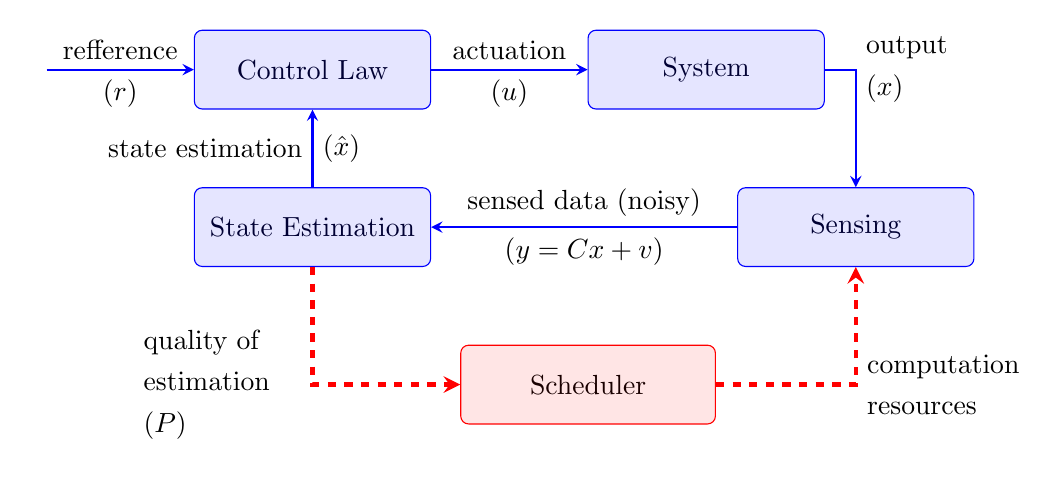
\begin{tikzpicture}[node distance=2cm]
        \node (in) [eNode] {};
        \node (control) [recNodeB, right of=in, xshift=1.5cm] {Control Law};
        \node (sys) [recNodeB, right of=control, xshift=3cm] {System};
        \node (sensor) [recNodeB, below of=sys, xshift=1.9cm] {Sensing};
        \node (estimator) [recNodeB, below of=control] {State Estimation};
        \node (sched) [recNodeG, below of=estimator, xshift=3.5cm, text width=3cm] {Scheduler};
        
        \draw [arrowB] (in) -- node[above] {refference} node[below] {($r$)} (control);
        \draw [arrowB] (control) -- node[above] {actuation} node[below] {($u$)} (sys);
        \draw [arrowB] (sys) -| node[right,text width=1cm] {output ($x$)} (sensor);
        \draw [arrowB] (sensor) -- node[above] {sensed data (noisy)} node[below] {$(y = Cx +v$)} (estimator);
        \draw [arrowB] (estimator) -- node[left] {state estimation} node[right] {($\hat{x}$)} (control);
        
        \draw [arrowG] (sched) -| node[right,text width=2cm] {computation resources} (sensor);
        %\draw [arrowG] (sched) --  node[right] {$var(v)$} (estimator);
        \draw [arrowG] (estimator) |- node[left,text width=2cm] {quality of estimation ($P$)} (sched);
        
        
        \end{tikzpicture}
        
        \caption{A general scheduling framework. Each control loop (depicted in blue) informs the resource allocator (Scheduler) of its quality of estimation and the allocator allocates accordingly the computation resources among all the control loops, in order to maintain valid estimation quality. 
            %The underlying assumption here is that the noise in the sensed data is a function of the amount of computation resources. We assume that the more resources are invested in sensing the better (less noisy) sensed data is obtained.
            \label{fig:general_hybrid_loop}}
    \end{figure}
    
    \begin{figure}[h]
        \centering
        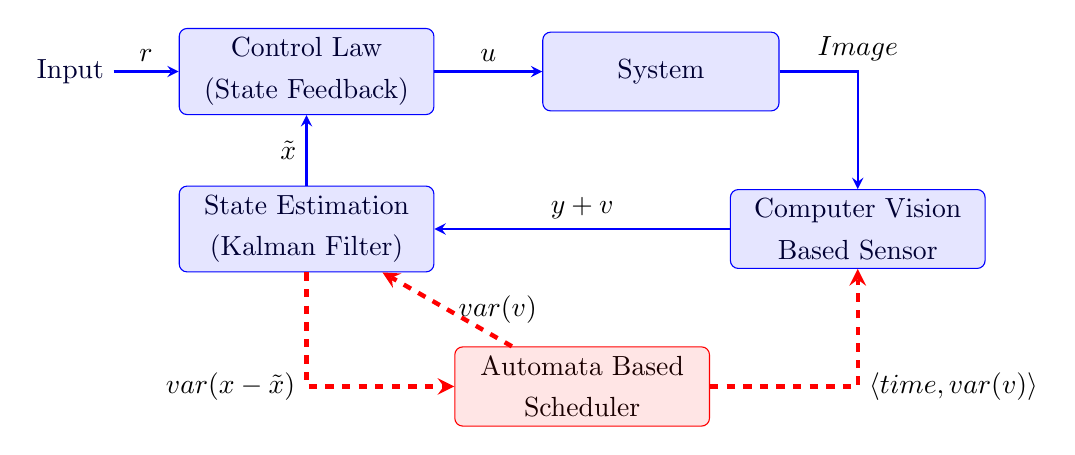
\begin{tikzpicture}[node distance=2cm]
        \node (in) [eNode] {Input};
        \node (control) [recNodeB, right of=in, xshift=1cm, text width=3cm] 
        {Control Law (State Feedback)};
        \node (sys) [recNodeB, right of=control, xshift=2.5cm] {System};
        \node (sensor) [recNodeB, below of=sys, xshift=2.5cm, text width=3cm] 
        {Computer Vision Based Sensor};
        \node (estimator) [recNodeB, below of=control, text width=3cm] 
        {State Estimation (Kalman Filter)};
        \node (sched) [recNodeG, below of=estimator, xshift=3.5cm, text width=3cm] {Automata Based Scheduler};
        
        \draw [arrowB] (in) -- node[above] {$r$} (control);
        \draw [arrowB] (control) -- node[above] {$u$} (sys);
        \draw [arrowB] (sys) -| node[above] {$Image$} (sensor);
        \draw [arrowB] (sensor) -- node[above] {$y+v$} (estimator);
        \draw [arrowB] (estimator) -- node[left] {$\tilde{x}$} (control);
        
        \draw [arrowG] (sched) -| node[right] {$\langle time,var(v) \rangle$} (sensor);
        \draw [arrowG] (sched) --  node[right] {$var(v)$} (estimator);
        \draw [arrowG] (estimator) |- node[left] {$var(x-\tilde{x})$} (sched);
        
        \end{tikzpicture}
        
        \caption{The controller framework we will implement, the \textit{scheduler} will allocate CPU time ($\langle time,var(v) \rangle$) for the \textit{Computer Vision} task base on the state estimation certainty using guarded Automata.
            \label{fig:hybrid_loop}}
    \end{figure}
    
}

%TODO - probably need to be in the Tests section
TODO - need to fix here!!!
\commentOut{
    As shown in Figure~\ref{fig:hybrid_loop}, the system framework consists of an interaction between the scheduler and the control loops, in this case the estimator (\textit{State~Estimator}) accuracy strongly depends on the sensing task (\textit{Computer~Vision}) and they both collaborate with the \textit{scheduler} in order to achieve their \textbf{control objectives} (g.e. stability).
    In this framework the scheduler is part of the control logic and therefore it can make scheduling decisions based on the current control state, the scheduling of \textit{Computer~Vision} task depends on the accuracy of state estimation.
    For example, if the vision is clear, the \textit{Computer~Vision} will produce good measurement of the \textit{System} and therefore good accuracy will be achieved so the \textit{Scheduler} can allocate less computation time to the heavy \textit{Computer~Vision} task and still remain stable while allocating more CPU to others control loops or to background tasks (like navigation).
    
    We will use an existing open-source implementation of drone software as a basis for our experimentation. However, the above collaboration requires to re-adjust some parts of the control system, e.g. the \textit{State~Estimator} needs to work with variable error variance of \textit{Computer~Vision} measurement,  the \textit{Computer~Vision} needs to be able run within variable time limits, and the tasks pre-defined requirements need to be re-adjusted in order to define the relation between tasks such as \textit{Computer~Vision} and \textit{State~Estimator}.
}

% TODO - make some connection
Below we will dive in each part of the new architecture and explain how it should be adjusted.

\subsection{Sensors}
\label{sec:sensors}
The sensing process are assumed to be periodic task. 
In order to allow dynamic scheduling it must be able to execute in a variable period between executions or to allow control of the execution duration time.
There are two general approaches we consider for this task: use \textit{any-time} algorithms or finite \textit{execution-modes} based tasks.
\textit{any-time} algorithms are algorithms that always try to improve the solution quality, for sensing processes, we can define deadline for the ``searching" process every execution, ??? present any-time solution for image processing~\cite{Shlomo}.
%TODO - "its also can be apllyed to general task by avaraging berst of exeqution in short time
%TODO also used by "anytime"
%TODO contract-based
Set of \textit{execution-modes} based, a discrete version influence from ``contract-based'' presented by ??? Pant~\cite{UPenn-Pant}, here each sensing task have finite number of ``operation modes'', e.g. different algorithms to proximate the same observations value, then the scheduler can perform the apropriate mode for every cycle.

For simplicity, we only work with \textit{execution-modes} based sensing tasks, all the modes are pre-defined and identified by a pair $\langle Duration, Variance \rangle$,
which define the error $Variance$ of this mode and the run-time $Duration$ is the of this mode. 
We assume that longer modes produce solution with smaller error variance.
%TODO - reed a litle the article (\cite{UPenn-Pant}) and re-write the next.
%TODO - check if Anitime reserch (\cite{Shlomo}) can fit here.
%TODO - Make sure that we use the terms contract-base and any-time correctly

\subsection{State Estimator}
\label{sec:estimator}
% kalman filter & ...
% seperation rule of kalman

State Estimator (the filter) is part of the estimation process, this unit receive the measurements ($y$) from the \textit{Sensors} and produce from them the state estimation required by the controller ($\hat{x}$).
When the \textit{Sensors} is accurate enough we may be able to pass it directly to the \textit{Controll Law} ($\hat{x} = y$), but usually the measurement is noisy and the main goal of the State Estimator is to reduce this noise from the measurement (see Section~\ref{sec:kalman}).
%TODO mybe add this: some times the sensor measure not mesure the needed state parameters, for example if we need to know the amount of water in the botle baut we only know the flow during all the rime we need to integrate in order to know the quantity.

If one consider using the optimal estimator Kalman filter (describe at Section~\ref{sec:kalman}) in the estimation process, one of the parameter that need to be consider in calculation is the covariance of sensor error (noted by $R$ in Section~\ref{sec:kalman}).
But in the new framework the sensor have diferents operation modes with variable error covariance, this means that we need to have also variable state estimators correspondingly.
In order to adjust the sensor error covariance, each cycle the scheduler will inform the state estimator about the new error covariance, and the state estimator will use corresponding parameters to make the next estimation.
%TODO - if the next is included need to read and learn "time-variant kalman filter"
%The second parameter that may be problematic is the state evolution in time ($A$ matrix in KF), which is defined for specific time period, and need to be adjusted if we use variable period, or maybe use time-variant kalman filter.

\subsection{Control Tasks} 
\label{sec:control} 
The control task (regulator) itself (\textit{Control Law} in Figure~\ref{fig:general_hybrid_loop}) is responsible for closing the gap between current state estimation ($\hat{x}$) and the reference state ($r$), by manipulating the system actuators (e.g. changing the speed of the motors), that output to the actuators is noted by $u$.

%Optimal estimation or optimal control law is not guarantee the overall optimal feedback controller, but as Kalman prove, 
The control task is usually a very low CPU consumer and been well studied~\cite{Bennett,Cervin}. Hence, the control task is not needed to be manipulated.
For our testing we use the commonly used and well known technique from control theory called PID, A proportional-integral-derivative controller.
In this technique the control output is based on the physical knowledge of the system dynamics, and have three variable parameters (P, I and D) that define the controller convergence behavior \cite{PID} ???.

%TODO
\commentOut{
    We also plan to try to use an ``adjustable'' LQR (Linear-quadratic regulator) control, as follows.
    LQR is an optimal controller that take into account the level of certainty of the state estimation. 
    Is usually a hard task to know the certainty of estimation, but in our case we need to calculate it anyway, and we mark it as $var(x-\tilde{x})$.
    We will make LQR ``adjustable'' in the sense that each iteration the controller will consider the new (variable) $var(x-\tilde{x})$. This is similar to the architecture we proposed for the estimator.
    We will check if adjustable LQR has significant advantages over PID in cases were we have variable certainty of estimation.
}

\subsection{Computation Resource Scheduler: Automata Based Scheduler}
\label{sec:scheduler}

Real-time systems are mostly composed of multiple real-time tasks, tasks with time constraint, for example task that must response to an event within specified time constraints.
The purpose of schedulers in such systems is to allocate the limited computational resources (CPU time) within all the task in the system. To do so, we need a well defined interface between the real-time tasks and the scheduler.

The most common way of describing the requirements of a real-time component is to specify a period, sometimes along with a deadline, which gives the frequency at which the component must execute. 
The designer of the component makes sure that the performance objectives are met as long as the component is executed consistent with its period. The scheduler guarantees that all components get enough resources.
%not directly in this article
Specifying resource requirements using periods has advantages due to simplicity and analyzability, but has limited expressiveness, as elaborated in~\cite{RTComposer}. 
%For example, a specification such as “execute the component every 5ms” does not say whether the scheduler should or should not execute it more frequently if enough computing resources are available, and if a component has multiple methods, say, for different control tasks, each needing a different period, the requirement cannot be naturally captured by a single period.





% TODO - stop here!
\subsubsection{The Proposed Scheduling Methodology}
In this thesis we develop a new methodology for allocation resources. We focus on how should engineers describe the requirements of a real-time component.
To simplify, we will assume that the resource is allocated in discrete \textit{time slots} of fixed duration in the style of time-triggered architecture~\cite{RTComposer}.
%TODO - read again this section
%We will develop automata based (hybrid automata) methodologies and schedulers based on the work of Alur~\cite{RTComposer} and Bukra~\cite{Merav}, and will demonstrate with measurable data how they improve the performance of real flying drones (see Section~\ref{sec:results}).
The specification framework for resource requirements is based on \textit{Nondeterministic $\omega$-automata} (finite automata over infinite words)~\cite{???}.
Automata can be more expressive for describing specific requirements, and they are composable, i.e., it is easy to compose all the tasks requirements into an integrated automata, and its easy to analyze and manipulate using tools like GOAL~\cite{???}.


%TODO - what we do with $Acc$
Formally \textit{task specification automata} is defined, similarly to Nondeterministic $\omega$-automata, as tuple $A=(Q,\Sigma,\Delta,Q_0,Acc)$.
In our setting, the \textit{alphabet} of the automata is $\Sigma = T^2 \times C^2$ where 
$C$ is the set of Boolean conditions variables, will be describe later, and $T$ is the set of all tasks in the system.
Each infinite word ($\alpha \in \Sigma^\omega$) of the automata define a possible tasks scheduling over a fixed period (time slots), and the automata language define all the possible scheduling.
Now the scheduler only need to ``walk through'' the automata as follows, before every iteration (time slot) the scheduler choose state transition $(q_i , \{t_j , c_j\}, q_{i+1})$ from the current state $q_i$ to the state $q_{i+1}$


Let's define $s()$









%Hybrid automata is a variation of finite automata for real-valued continuously progressing words~\cite{hibrid-systems}.
In our setting, the automata define continuous (fixed period) operation modes, and the condition of mode changing.
The operation mode directly define a set of tasks that will be executed in the time slot (for example $s_{0.7}$ in Figure~\ref{fig:sched_sense_auto}).
We can stay at a single mode for some iterations, in this case the same tasks will be scheduled in each iteration. 
We can also take \textbf{discrete mode transition} in order to change operation mode after few iterations and schedule different set of tasks, for example, in Figure~\ref{fig:sched_sense_auto} the edge $(m_1,m_2)$ says that if the previous iteration mode was $m_1$ and $estVar < 0.7$ we can change the mode and schedule the set $\{s_{0.2}\}$ in the next iteration.

Each infinite path on the composed hybrid automata (not necessarily with infinitely many mode transitions) represents a schedule that satisfy all the tasks requirements. 
In this architecture the scheduler only need to ``walk through'' the composed automata, this is, of course, a fast and easy computational task. 
In order to assure that we do not exceed the time slot duration, each task will have pre-defined maximum duration time like ``deadline'' in the traditional architecture. Now we can verify that every possible scheduling step can execute within a single time slot, in other words, every mode of the composed automata can be executed in a single time slot, by simply summing the ``deadlines'' of all the tasks in the mode tasks set.
%we can summarize the total slot ``deadline'' as follows:\\
%$\forall mode~e ~~(\sum_{t \in Guard(e)} deadline(t) ) \leq slot~duration$ \\
If we find a mode that goes beyond the maximum duration we can remove it from the automata so we never exceed the time slot duration.


\begin{figure}[]
    \centering
    
    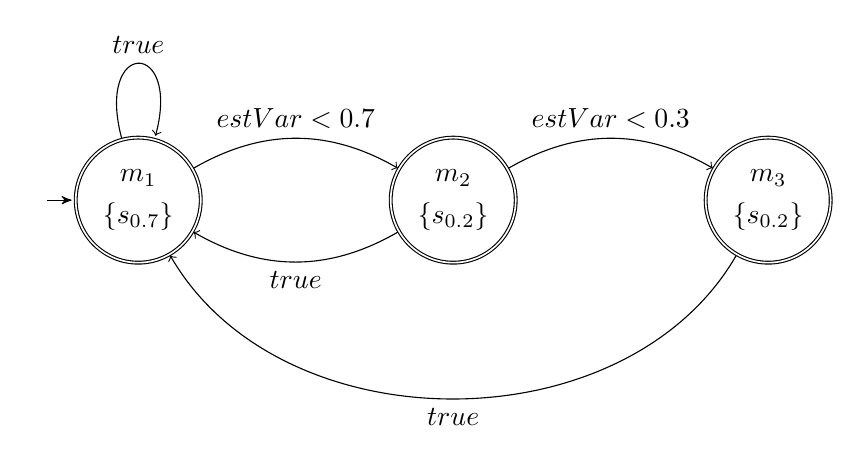
\begin{tikzpicture}[node distance=4cm, text centered, auto]
    \node (A) [state, accepting, text width=1cm, initial] {$m_1$ $\{s_{0.7}\}$};
    \node (B) [state, accepting, text width=1cm] [right of=A] {$m_2$ $\{s_{0.2}\}$};
    \node (C) [state, accepting, text width=1cm] [right of=B] {$m_3$ $\{s_{0.2}\}$};
    
    \path[->] (A) edge [loop above] node {$true$} (A);
    %\path[->] (A) edge [bend left] node {$\neg est_{bad} \wedge s_{0.2}$} (B);
    \path[->] (A) edge [bend left] node {$estVar < 0.7$} (B);
    \path[->] (B) edge [bend left] node {$true$} (A);
    %\path[->] (B) edge [loop above] node {$\neg var3$} (B);
    %\path[->] (B) edge [bend left] node {$est_{good} \wedge s_{0.2}$} (C);
    \path[->] (B) edge [bend left] node {$ estVar < 0.3$} (C);
    %\path[->] (C) edge [loop above] node {$var1$} (C);
    \path[->] (C) edge [bend left=60] node {$true$} (A);
    
    
    \end{tikzpicture}
    
    \caption{Example of guarded automata for our vision based sensor task, in this example the task has two operation modes, $\mathbf{s_{0.7}}$ which need 70\% of the time slot but is more accurate vision computation and $\mathbf{s_{0.2}}$ which is less accurate but faster (need only 20\% of the slot).
        The value of $estVar$ is $var(x-\tilde{x})$ of the previous iteration.
        Every time slot exactly one of the modes will be executed.
        \label{fig:sched_sense_auto}}
\end{figure}

\begin{figure}[]
    \centering
    
    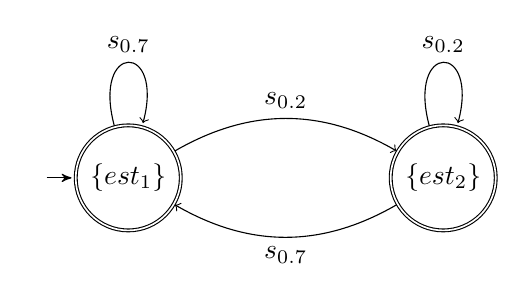
\begin{tikzpicture}[node distance=4cm,auto]
    \node (A) [state, accepting, initial] {$\{est_1\}$};
    \node (B) [state, accepting] [right of=A] {$\{est_2\}$};
    
    \path[->] (A) edge [loop above] node {$s_{0.7}$} (A);
    \path[->] (B) edge [bend left] node {$s_{0.7}$} (A);
    %\path[->] (A) edge [bend left] node {$s_{0.2} \wedge est_2$} (B);
    %\path[->] (B) edge [loop above] node {$s_{0.2} \wedge est_2$} (B);
    \path[->] (A) edge [bend left] node {$s_{0.2}$} (B);
    \path[->] (B) edge [loop above] node {$s_{0.2}$} (B);
    %\path[->] (B) edge [bend left] node {$s_{0.7} \wedge est_1$} (A);
    
    \end{tikzpicture}
    
    \caption{Example of guarded automata for our state estimator, in this example the estimator has two operation modes, $\mathbf{est_1}$ correspond to $\mathbf{s_{0.7}}$ and $\mathbf{est_2}$ correspond to $\mathbf{s_{0.2}}$~(see Figure \ref{fig:sched_sense_auto}).
        \label{fig:sched_estimator_auto}}
\end{figure}

Let us demonstrate the proposed automata based interface using the system depicted in Figure~\ref{fig:hybrid_loop}.
Assume we have two operation modes of the vision based sensor: (1) $s_{0.7}$ a very accurate operation mode that takes 70\% of the time slot to execute, that is of course a significant amount of time, and (2) $s_{0.2}$ a less accurate operation mode but takes only 20\% of the slot.
In each time slot we can execute one of them and get the sensing process done, but if we use only $s_{0.7}$ every time slot we may not have enough time to execute all the tasks. On the other hand, if we use only $s_{0.2}$ we will have inferior estimates.
Figure~\ref{fig:sched_sense_auto} shows an example of a guarded automata that guides the schedule. With this automata we can express rich specifications. 
In this example, execute $s_{0.7}$ is always allowed but if we need faster sensing we can use $s_{0.2}$ but only once in a row if the estimation error is not extremely bad~(if~$var(x-\tilde{x}) < 0.7$), or even twice in a row if the estimation error is good~(if~$var(x-\tilde{x}) < 0.3$).

The estimated estimation error ($estVar$ in the figure) is, in this case, the estimation error variance ($var(x-\tilde{x})$ in Figure~\ref{fig:hybrid_loop}). 
%if $var(x-\tilde{x})$ is small then $est_{good} = true$, if is normal then $est_{normal} = true$ end $est_{bad} = true$ if $var(x-\tilde{x})$ is  bigger then some boundary.
\\This value ($estVar~=~var(x~-~\tilde{x})$) is calculated by the state estimator task (Section~\ref{sec:estimator}) and is passed to the scheduler as discussed before.

Each of this operation modes ($s_{0.7}$ and $s_{0.2}$) have different accuracy, specified by $var(v)$ in Figure~\ref{fig:hybrid_loop}, and if we want to get optimal estimation the state estimator mast be configure correspondingly, i.e., the sensing error variance should be adjusted to the correct value ($var(s_{0.7})$), an easy solution for specifying the different configurations is by the guarded automata shown in Figure~\ref{fig:sched_estimator_auto}, which defines two operation modes of the state estimator, $est_1$ and $est_2$, that correspond to $var(s_{0.7})$ and $var(s_{0.2})$. So of course if we sense in mode $s_{0.7}$ we must estimate with mode $est_1$ that has the correct configurations for $s_{0.7}$, and if we sense in mode $s_{0.2}$ we must estimate with mode $est_2$.    
}

%\begin{samepage}
\bibliographystyle{abbrv}
\bibliography{hodai_thesis}
%\end{samepage}

\begin{titlepage}
    \hspace{3cm}
\end{titlepage}

%\includepdf[pages={1-}]{./Chapters/HebrewPages.pdf}
\todo[inline]{Need to update the hebrew pages}

\end{document}}